%
% Copyright (c) 2017  Zubax Robotics OU  <info@zubax.com>
%
% Distributed under BY-NC-ND (attribution required, non-commercial use only, no derivatives).
%

\documentclass{zubaxdoc}
\graphicspath{{document_templates/documentation_template_latex/}}

\usepackage{ConfigParamIndex}
\usepackage{amsmath}
\usepackage{textcomp}

\title{Zubax GNSS 2 Datasheet}

\hbadness=10000

\begin{document}
\frontmatter

\begin{titlepage}

\section*{Overview}

Zubax~GNSS~2 is a multipurpose high-performance positioning module interfaced via CAN bus, USB, and UART.
It includes a state-of-the-art multi-system GPS/\allowbreak{}GLONASS receiver,
a high-precision barometric altimeter, and a 3-axis compass with thermal compensation.

\section*{Features}

\begin{itemize}
    \item State-of-the-art concurrent GPS/GLONASS receiver u-blox MAX-M8Q.
    \begin{itemize}
    	\item Full RF shielding of the GNSS circuits ensures reliable operation in high-EMI environments.
    	\item 35 mm high-gain patch antenna with large ground plane for reliable reception even in deep urban canyons.
    	\item Analog front-end with LNA and SAW ensures high noise resilience.
    	\item Supercapacitor-based backup power source enables low time-to-first-fix (a few seconds).
    	\item Up to 15 Hz update rate.
    \end{itemize}
	\item High precision digital barometer TE Connectivity MS5611.
    \item High precision 3-axis digital compass STMicroelectronics LIS3MDL with thermal compensation.
	\item Supported interfaces:
    \begin{itemize}
        \item CAN, with optional dual redundancy.
        \item UART.
        \item USB port, no drivers needed.
    \end{itemize}
    \item High quality assurance:
    \begin{itemize}
        \item Every manufactured unit undergoes a strict testing procedure.
        The testing log for each produced unit is available to the user via the website at
        \url{https://device.zubax.com/device_info}.
        \item Protection against unlicensed (counterfeit) production by means of a digital signature
        installed on every manufactured unit.
    \end{itemize}
\end{itemize}

\BeginRightColumn

\section*{Applications}

\begin{itemize}
	\item Positioning module for unmanned vehicles (aerial, ground, underwater, etc) and robots.
    \item General-purpose embedded positioning module.
\end{itemize}

\centering
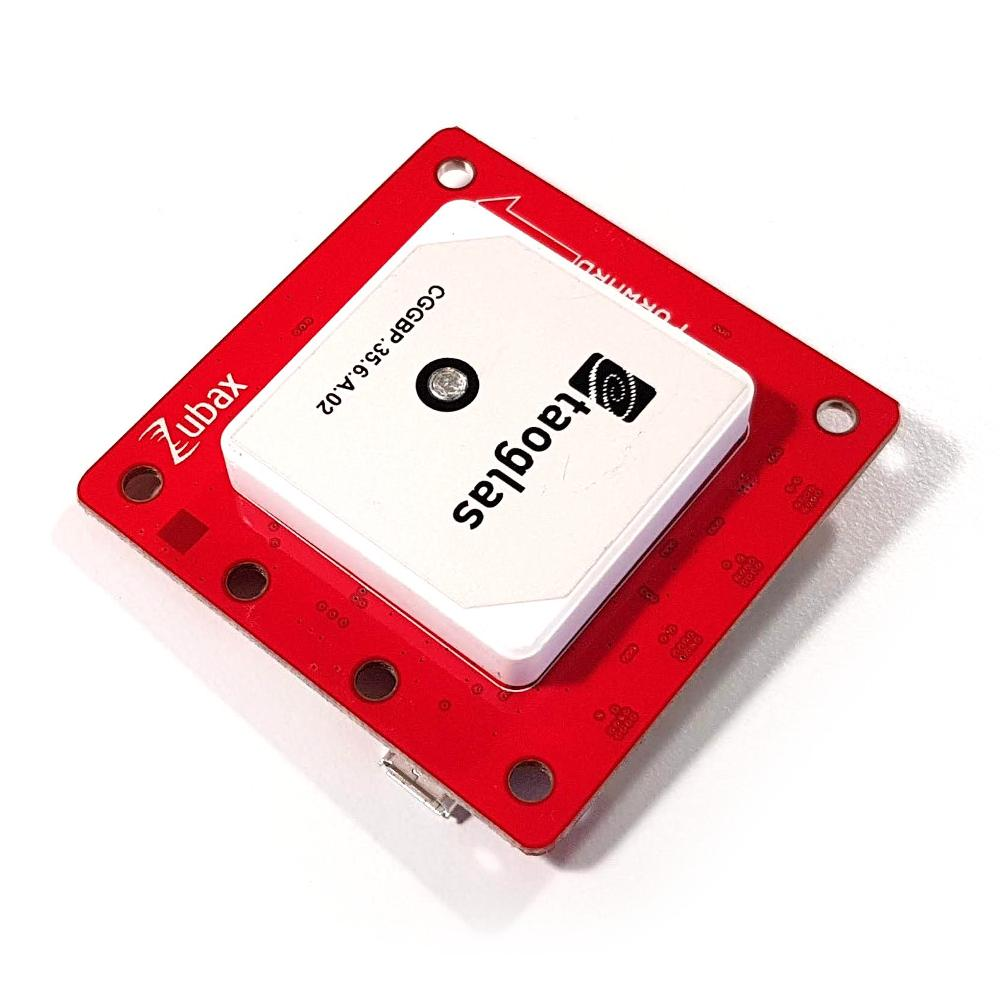
\includegraphics[width=0.45\textwidth]{GNSS_top}
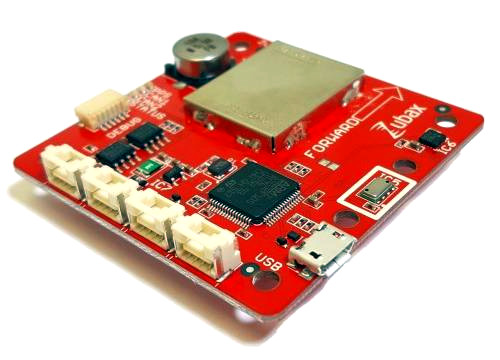
\includegraphics[width=0.45\textwidth]{GNSS_bottom}
\end{titlepage}

\tableofcontents
\listoffigures
\listoftables

\mainmatter

\chapter{Overview}

Zubax~GNSS~2 is a multipurpose high-performance positioning module interfaced via CAN bus, USB, and UART.
It includes a state-of-the-art multi-system GPS/GLONASS receiver,
a high-precision barometric altimeter, and a 3-axis compass with thermal compensation.
Zubax~GNSS~2 supports a variety of standard protocols,
which ensures compatibility with third party software and hardware:
UAVCAN (over CAN bus), NMEA 0183 (over USB and UART), and the u-Blox M8 binary protocol.

\section{Accessories}

Zubax~GNSS~2 can be used with the following accessories:

\begin{itemize}
    \item Plastic enclosure described in the section \ref{sec:enclosure}.
    \item UAVCAN cabling and related items.
    \item Standard USB cables.
    \item Cables compatible with the Dronecode Autopilot Connector Standard.
\end{itemize}

Please contact your supplier for ordering information.

\subsection{Enclosure}\label{sec:enclosure}

Zubax~GNSS~2 is intended for integration into the end system in the form of the bare PCB,
as this facilitates lower weight and tighter arrangement of components
in the end device, all of which are desirable properties in the targeted application domains.

Shall it be desired to provide additional mechanical protection for the device
or to install it away from possible sources of electromagnetic interference,
the plastic components pictured on the figure \ref{enclosure} can be used.
Please contact your supplier for the ordering information;
alternatively, visit \url{https://github.com/Zubax/zubax_gnss} to download
the 3D printable models suitable for in-house manufacturing.

\begin{figure}[hbt]
	\centering
	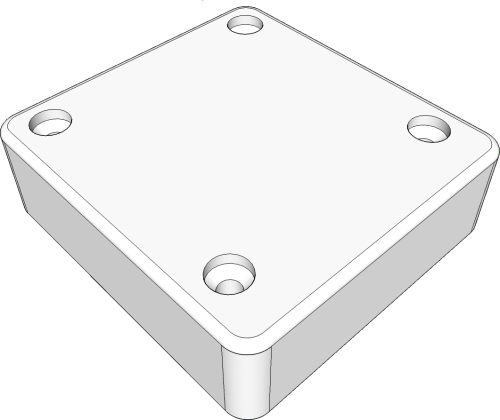
\includegraphics[width=0.45\textwidth]{enclosure_assembled_top}
	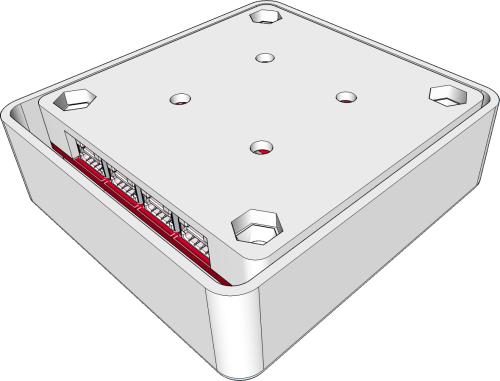
\includegraphics[width=0.45\textwidth]{enclosure_assembled_bottom}
	\caption{Plastic enclosure suitable for 3D-printing, top and bottom, assembled.\label{enclosure}}
\end{figure}

\begin{figure}[hbt]
	\centering
	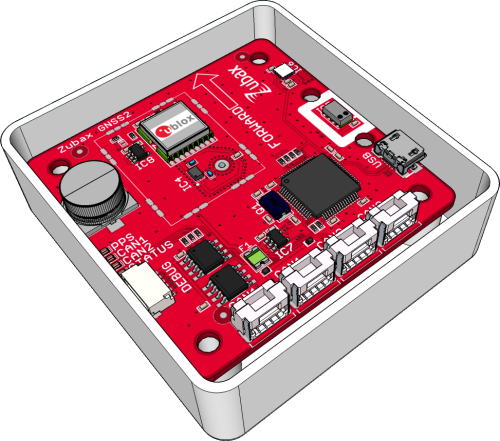
\includegraphics[width=0.45\textwidth]{enclosure_pcb_top}
	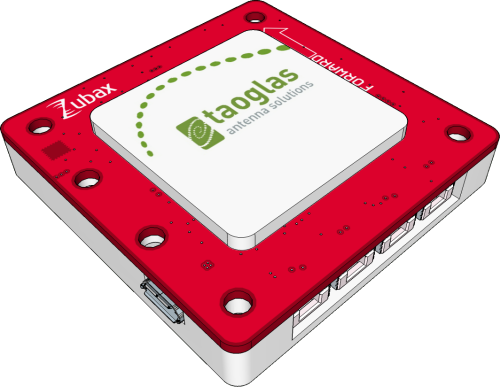
\includegraphics[width=0.45\textwidth]{enclosure_pcb_bottom}
	\caption{Top and bottom parts of the enclosure with the device inside.}
\end{figure}

\section{Quality assurance}

Every manufactured Zubax~GNSS~2 undergoes an automated testing procedure that validates that
the device is functioning as designed.
The test log for every manufactured device is available on the web at
\url{https://device.zubax.com/device_info}.
This feature can be used to facilitate traceability of purchased devices and
provide additional safety assurances.

Every manufactured device has a strong digital signature stored in its non-volatile memory
which proves the origins of the product and eliminates the risk of sourcing unlicensed or
counterfeit hardware.
This signature is referred to as Certificate of Authenticity (CoA).
Please refer to the \href{https://kb.zubax.com}{Zubax Knowledge Base} to learn more about
the certificate of authenticity and how it can be used to trace the origins of your hardware.

\chapter{Characteristics}

\section{Absolute maximum ratings}

Stresses that exceed the limits specified in this section may cause permanent damage to the device.
Proper operation of the device within the limits specified in this section is not implied.

\begin{ZubaxSimpleTable}{Absolute maximum ratings}{|c X|c c|c|}
    Symbol            & Parameter                & Min  & Max & Unit \\
	$V_\text{supply}$ & Supply voltage           & -0.3 & 6   & V \\
	$T_\text{oper}$   & Operating temperature    & -40  & 85  & \degree{}C \\
	                  & UART input voltage 		 & -0.3 & 6   & V\\
	                  & CAN H/L input voltage    & -4   & 16  & V\\
\end{ZubaxSimpleTable}

\section{Environmental conditions}\label{environmental_conditions}

The GNSS hot start feature is not expected to work reliably below -20\degree{}C
due to degraded performance of the supercapacitor-based backup power source at low temperatures.
However, this should not have any adverse side effects on the general performance of
the unit except that the time-to-first-fix (TTFF) may be higher than normal.

Magnetic fields whose magnitude exceeds the limit may render the compass temporarily dysfunctional.
Other components are unlikely to be affected.

\begin{ZubaxTableWrapper}{Environmental conditions}
    \begin{ZubaxWrappedTable}{|c X|l c|c|c|}
        Symbol            & Parameter                     &  Min & Max & Unit \\
        $T_\text{oper}$   & Operating temperature         & -40  & 85  & \degree{}C \\
        $T_\text{stor}$   & Storage temperature           & -20  & 60  & \degree{}C \\
        $B$               & Magnetic field strength       &      & 9   & Gauss \\
        $\phi_\text{oper}$& Operating humidity\tnote{1}   & 0    & 100 & \%RH\\
        $h_\text{oper}$   & Operating altitude above mean sea level (MSL) &     & 10  & km\\
    \end{ZubaxWrappedTable}
    \begin{tablenotes}
        \item[1] Condensation not permitted.
    \end{tablenotes}
\end{ZubaxTableWrapper}

\section{Reliability}

Please contact Zubax Robotics for additional reliability and safety information.

\begin{ZubaxSimpleTable}{Reliability}{|c X|c|c|}
    Symbol & Parameter & Typ & Unit \\
	MTTF   & Mean time to failure & 500000 & hours \\
\end{ZubaxSimpleTable}

\section{Sensor suite}

\subsection{GNSS receiver}

The device employs the \textbf{u-Blox MAX-M8Q} GNSS receiver module.
Please refer to the specifications provided by u-Blox to gain additional information about the module.

The cumulative delay (lag) of GNSS data is approximately 200 milliseconds,
not including the latency of the output interface.

The period of GNSS solution reporting is defined by the configuration parameters
\CfgRef{uavcan.pubp-fix} and \CfgRef{uavcan.pubp-aux}, in microseconds.

The parameters \CfgRef{gnss.warn+dimens} and \CfgRef{gnss.warn+sats} can be used to reflect the quality of
the GNSS solution in the device health code (section \ref{sec:self-diagnostics}).

\subsection{Digital barometric altimeter}

The device employs the \textbf{TE Connectivity MS5611} digital barometric altimeter.
Please refer to the specifications provided by TE Connectivity to gain additional information about the sensor.

The measurement period (which equals the reporting period) is defined by the configuration parameter 
\CfgRef{uavcan.pubp-pres}, in microseconds.
The reported error variances for pressure and temperature estimates are defined by the parameters
\CfgRef{pres.variance}, in $\text{pascal}^2$, and \CfgRef{temp.variance}, in $\text{kelvin}^2$,
respectively.

If the board is mounted in an open air environment, it is recommended to cover the sensor with a lid
in order to avoid distortions of the atmospheric pressure measurements caused by the movement of air
around the sensor.
Please refer to your supplier for additional information.

This sensor is also used for measuring the temperature of the air.
Due to the heat dissipated by the board,
the measured air temperature may be offset by up to +5 kelvin.

\subsection{Three-axis digital compass with thermal compensation}

The device employs the \textbf{STMicroelectronics LIS3MDL} digital three-axis compass with thermal compensation.
Please refer to the specifications provided by STMicroelectronics to gain additional information about the sensor.

Zubax GNSS v2.1 and older (manufacturing years 2015--2016) used to employ \textbf{Honeywell HMC5983} instead.
These modifications of the hardware are no longer manufactured.

The measurement period (which equals the reporting period) is defined by the configuration parameter 
\CfgRef{uavcan.pubp-mag}, in microseconds.
The reported error variance for magnetic field strength measurements is defined by the parameter
\CfgRef{mag.variance}, in $\text{gauss}^2$.

The measured magnetic field vector can be rescaled with the help of the parameter \CfgRef{mag.scaling+coef}.
This feature can be used to work-around magnetic field scaling issues in some commercial UAV autopilots.

The parameter \CfgRef{mag.pwron+slftst} can be used to control whether the magnetic field sensor should be
subjected to a self-test when the device is powered on.\footnote{Available for hardware v2.2 and newer.}
This feature should be disabled if the device is expected to be powered on while non-stationary,
otherwise false failures may be detected.

\section{Communication interfaces}

Zubax~GNSS~2 features three communication interfaces. Each is described in detail in the subsequent parts of this document.
\begin {itemize}
\item Doubly redundant UAVCAN interface with two connectors per interface.
\item USB port.
\item Dronecode port.
\end{itemize}

\subsection{CAN bus interface}

This interface provides full access to all features of Zubax~GNSS~2, including the output of measurements,
reconfiguration, time synchronization, firmware update, etc.

Zubax~GNSS~2 is equipped with a doubly-redundant CAN bus interface, which can be used in the non-redundant mode
as well.
Each of the interfaces is equipped with two standard
UAVCAN Micro connectors (JST GH)\footnote{\url{https://kb.zubax.com/x/EoAh}}
electrically parallel to each other,
which facilitates easy integration of the device into the end application without the need to use T-connectors.

The physical location of each connector is documented in the section \ref{sec:mechanical}.

\subsubsection{Device interconnection}

Zubax~GNSS~2 can be used with doubly-redundant and non-redundant CAN buses.
In the latter case, only CAN1 can be used, and CAN2 must be left unconnected.
The figure \ref{can_daisy_chain} shows the possible device interconnection schemes.

\begin{figure}[hbt]
    \center
	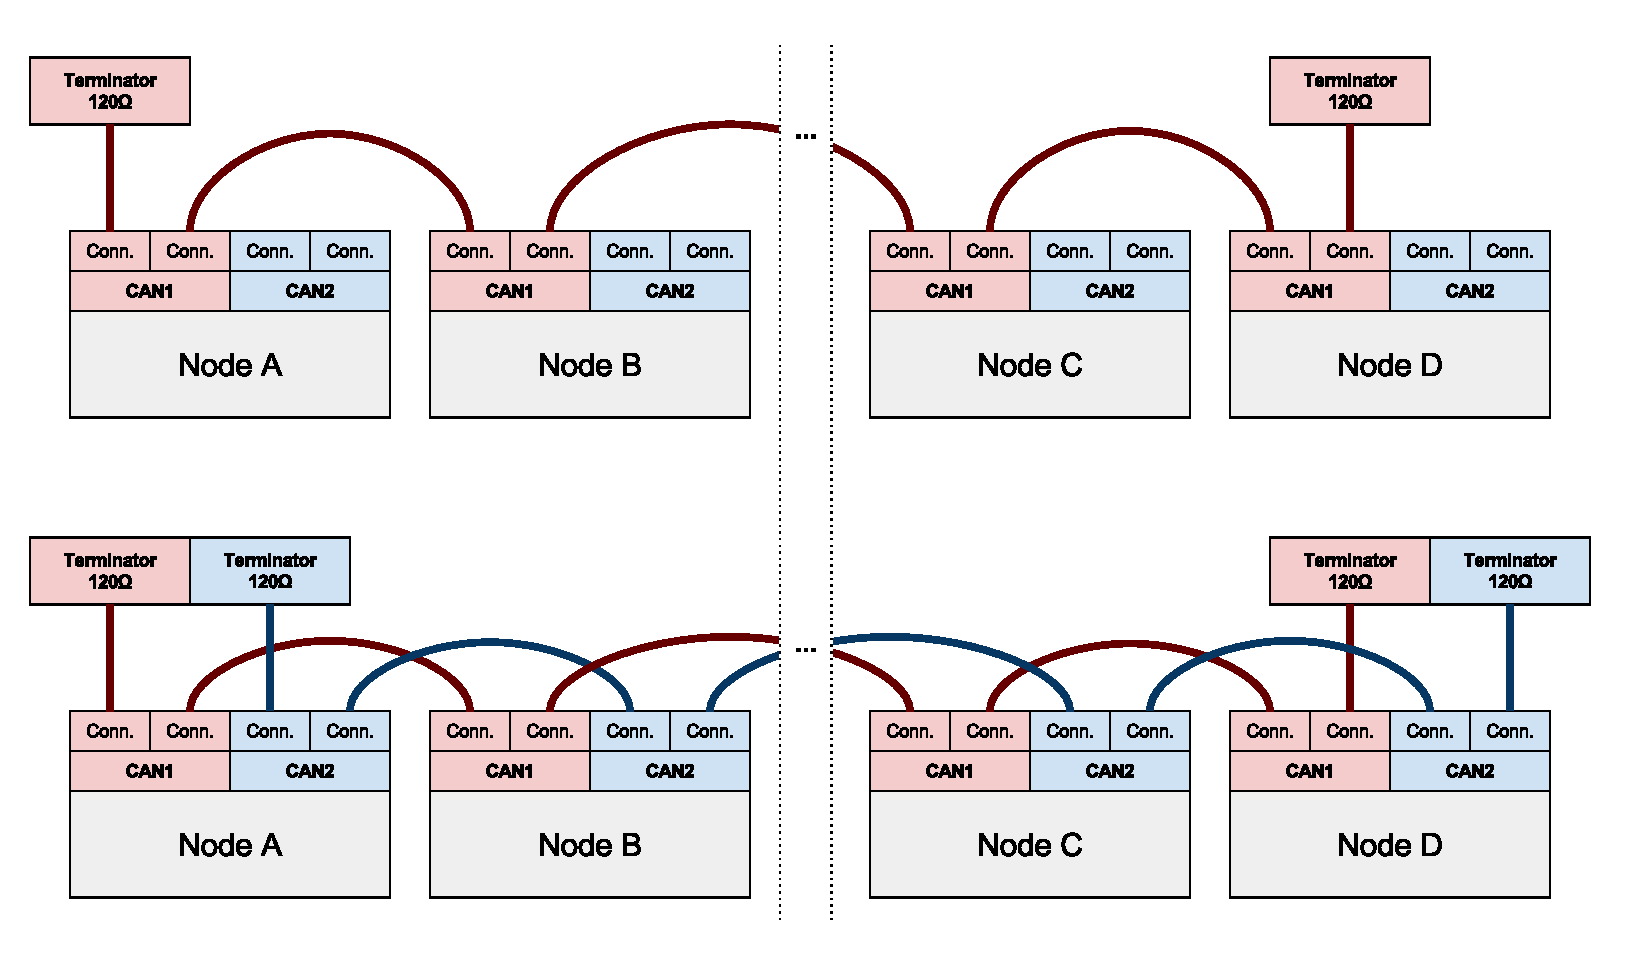
\includegraphics[width=1\textwidth]{can_daisy_chain}
	\caption{CAN bus interconnection diagram for non-redundant and a doubly-redundant interfaces.
	\label{can_daisy_chain}}
\end{figure}

\subsubsection{Connector pinout}

\begin{ZubaxTableWrapper}{UAVCAN Micro (JST GH) standard connector pinout}
    \begin{ZubaxWrappedTable}{|l X X[2]|}
        Pin no. & Type            & Function\\
        1       & Power           & +5 V power supply input and pass-trough\\
        2       & Input/output    & CAN High\\
        3       & Input/output    & CAN Low\\
        4       & Ground          & Power \& signal ground\\
    \end{ZubaxWrappedTable}
\end{ZubaxTableWrapper}

\subsubsection{Physical characteristics}

\begin{ZubaxTableWrapper}{Characteristics of CAN bus interfaces}
	\begin{ZubaxWrappedTable}{|c X|c c c|c|}
		Symbol  & Parameter                                 & Min  & Typ  & Max  & Unit \\
		        & Bit rate                                  &      &      & 1000 & Kbps \\
		        & Positive-going input threshold voltage    &      & 750  & 900  & mV \\
		        & Negative-going input threshold voltage    & 500  & 600  &      & mV \\
		        & Differential output voltage, dominant     & 1.5  & 2.0  & 3.0  & V \\
		        & Differential output voltage, recessive    & -120 & 0    & 12   & mV \\
		        & Inter-connector current pass-through\tnote{1}& -1&      & 1    & A \\
		        & Connector resistance during device lifetime &    & 30   & 50   & $\text{m}\Omega$ \\
	\end{ZubaxWrappedTable}
	\begin{tablenotes}
	    \item [1] The limit is imposed by the PCB.
	\end{tablenotes}
\end{ZubaxTableWrapper}

\subsection{USB interface}

The device implements a full-speed USB 2.0 port with the standard CDC ACM interface
(also known as ``virtual serial port'').
The device features driverless compatibility with all major operating systems
(Windows, GNU/Linux, Mac OS).\footnote{Get more knowledge and helpful tips at \url{https://kb.zubax.com}.}

The physical connector type is USB micro B (which is the most common device-side USB connector type).

\subsubsection{Identification}

Zubax~GNSS~2 will report the following properties to the USB host:
\begin{itemize}
    \item Vendor ID -- 0x1D50
    \item Product ID -- 0x60C7
    \item Vendor string -- \verb|Zubax Robotics|
    \item Device description string -- \verb|Zubax GNSS|
    \item Device ID -- the 128-bit globally unique device ID (section \ref{sec:product_identification})
                       as a hexadecimal string
\end{itemize}

\subsubsection{Protocol selection}\label{sec:usb_protocol_selection}

The following protocols are exposed via the USB interface:
\begin{description}

    \item[NMEA 0183] Used to output measurements in the industry-standard NMEA 0183 protocol.
    This protocol is enabled only if the virtual serial port is opened with a baud rate value in the
    range from 4800 to 57600 baud/second, inclusive.
    More information about the NMEA protocol is provided in the chapter \ref{nmea_output}.

    \item[CLI] The command-line interface provides access to the device's management and diagnostic
    features. This protocol is always enabled; however, it is not expected to be practically useful
    while used in parallel with other protocols, such as NMEA.
    More information about the CLI is provided in the section \ref{command-line_interface}.

\end{description}

Observe that unlike many other implementations of virtual serial ports,
this implementation is sensitive to the baud rate setting,
because it is used by the device to decide whether the NMEA output should be enabled.
The rationale behind this logic is to facilitate compatibility with third party software products.

Many legacy GNSS receivers equipped with physical UART interfaces emit NMEA data at very low
baud rates, typically between 4800 and 57600 baud/second.
This formed a widely used convention that when a client application needs to establish a connection
with an NMEA provider, it would first try a low speed, usually starting from 4800 or 9600
baud/second.
This triggers Zubax~GNSS~2 to enable the desired NMEA output immediately,
ensuring quick and reliable auto-configuration.

Conversely, most other products by Zubax expose physical UART interfaces at the default baud rate
value of 115200 baud/second, hence the NMEA output is disabled automatically when the port is opened at
this speed in order to ensure compatibility with other Zubax products.

\subsection{Dronecode debug port interface}

The device features a Dronecode debug port interface available via the standard
Dronecode Debug Mini connector (DCD-Mini)\footnote{\url{https://wiki.dronecode.org/workgroup/connectors/start}}.
This port can be conveniently used with the \href{https://kb.zubax.com/x/iIAh}{Zubax Dronecode Probe},
or any other UART-capable hardware with a compatible connector.

The physical location of the connector is documented in the section \ref{sec:mechanical}.

The Dronecode debug port provides access to the UART and JTAG/SWD interfaces;
the latter is not designed for production use and therefore it is not documented here.

\subsubsection{UART interface}

The UART interface available within this port operates with the following settings,
which cannot be changed by the user:\footnote{
Same UART settings are used by most of other Zubax products.}
\begin{itemize}
    \item Baud rate -- 115200
    \item Word size -- 8 bit
    \item Parity control -- none
    \item Stop bits -- 1 bit
\end{itemize}

The following protocols are exposed via the UART interface:
\begin{description}

    \item[Debug and diagnostics output] Zubax~GNSS~2 prints human-readable debug and diagnostic messages
    via the UART interface of the Dronecode port.
    These can be used for troubleshooting purposes.

    \item[NMEA 0183] Used to output measurements in the industry-standard NMEA 0183 protocol.
    NMEA emission over the UART port is disabled by default;
    in order to enable it, set the configuration parameter \CfgRef{nmea.uart+on} to a non-zero value.
    More information about the NMEA protocol is provided in the chapter \ref{nmea_output}.

\end{description}

\subsubsection{Connector pinout}

\begin{ZubaxTableWrapper}{Dronecode Debug Mini standard connector pinout}
    \begin{ZubaxWrappedTable}{|l X X X[2]|}
        Pin no. & Type            & Name                & Comment\\
        1       & Power           & TPWR                & +5 V power supply input\tnote{1}\\
        2       & Output          & UART\_TX            & Collect the NMEA and diagnostic output here\\
        3       & Input           & UART\_RX            & Pulled down with a resistor\\
        4       & Input/Output    & SWDIO               & Not for production use\\
        5       & Input           & SWDCLK              & Not for production use\\
        6       & Ground          & GND                 & Power \& signal ground\\
    \end{ZubaxWrappedTable}
	\begin{tablenotes}
	    \item[1] Available in hardware v2.1 (manufacturing year 2015) and newer.
                 Older revisions of the hardware cannot be powered via the Dronecode debug port.
	\end{tablenotes}
\end{ZubaxTableWrapper}

\subsubsection{Electrical characteristics}

\begin{ZubaxSimpleTable}{Dronecode debug port characteristics}{|c X|c c c|c|}
	Symbol  & Parameter                                 & Min  & Typ  & Max  & Unit \\
			& Low-level input voltage                   & -0.3 & 0    & 1.6  & V\\
			& High-level input voltage                  & 2.1  & 3.3  & 5.5  & V\\
			& Low-level output voltage                  & 0    & 0    & 0.5  & V\\
			& High-level output voltage                 & 2.8  & 3.3  & 3.4  & V\\
			& Source/sink current via data pins         &      &      & 10   & mA\\
			& UART RX pull down resistance              & 30   & 40   & 50   & $\text{k}\Omega$\\
	        & Connector resistance during device lifetime &    & 20   & 40   & $\text{m}\Omega$\\
\end{ZubaxSimpleTable}

\section{Power supply}

The device can be powered via the following inputs:
\begin {itemize}
\item Any single UAVCAN port.
\item Both UAVCAN ports simultaneously
(the power supply circuit prevents direct current flow between these power inputs).
\item USB port.
\item Dronecode port (hardware revisions v2.1 (year 2015) and newer).
\end{itemize}

It is allowed to power the device simultaneously via USB and UAVCAN, since the power supply circuits prevent back-powering via these interfaces.
It is not recommended to supply power via the Dronecode port while any other power input is used concurrently.

The power supply characteristics documented in the following table are invariant to the power input used.

\begin{ZubaxSimpleTable}{Power supply}{|c X|c c c|c|X|}
     Symbol             & Parameter      & Min & Typical & Max & Unit & Note \\
	 $V_\text{supply}$  & Supply voltage & 4.0 & 5.0     & 5.5 & V    & Any power input\\
	 $I_\text{supply}$  & Supply current & 70  & 95      & 180 & mA   & Any power input\\
\end{ZubaxSimpleTable}

\section{Product identification}\label{sec:product_identification}

This section documents the device properties that are reported in response to identification requests,
such as the UAVCAN service \verb|uavcan.protocol.GetNodeInfo| (section \ref{sec:uavcan_node_identification})
or the CLI command \verb|zubax_id| (section \ref{sec:cli_command_zubax_id}).

The product ID string and the UAVCAN node name are reported as ``\verb|com.zubax.gnss|''.
The prefix ``\verb|com.zubax.|'' is shared by many of the products designed by Zubax Robotics.

Every manufactured device has a globally unique 128-bit ID (UID) that cannot be changed.

Every manufactured device is equipped with a certificate of authenticity,
which is a function of, among other things, the UID and the product ID of the device.
Please refer to the web resources provided by Zubax Robotics to learn more about the certificate of authenticity
and how it can be used to verify the authenticity of products.

\subsection{Hardware and firmware versions}

The table \ref{table:product_revisions} summarizes the information about existing hardware revisions
and compatible firmware versions.
Note that all revisions of Zubax~GNSS~2 share the same major hardware version number~\textbf{2}.

\begin{ZubaxSimpleTable}{Zubax~GNSS product revision summary}{|l l l|X|}\label{table:product_revisions}
     Hardware                   & Year      & Firmware    & Notes                  \\
     \textbf{Zubax GNSS 1.0}    & 2014      & v1.x, v2.x  & First release. No longer manufactured. \\
     \textbf{Zubax GNSS 2.1}    & 2015      & v3.x        & Not backward-compatible with Zubax GNSS 1.0.
                                                            No longer manufactured. \\
     \textbf{Zubax GNSS 2.2}    & 2017      & v4.x        & Backward compatible with Zubax GNSS 2.1. \\
\end{ZubaxSimpleTable}

\section{Mechanical}\label{sec:mechanical}

The figure \ref{drawing} documents the basic mechanical characteristics of Zubax~GNSS~2,
such as the placement of connectors and mounting holes.

\begin{figure}[!hbt]
    \center
	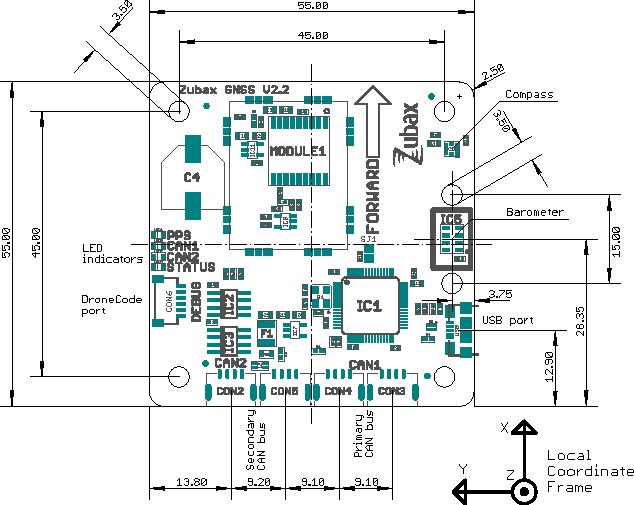
\includegraphics[width=1\textwidth]{GNSS2_drawing}
	\caption{Zubax GNSS 2 drawing.\label{drawing}}
\end{figure}

\chapter{Operating principles}

\section{Overview}

Zubax~GNSS~2 continuously reads measurements from active sensors and reports them via
active communication interfaces.
The GNSS receiver and the compass are always active,
whereas the air pressure and temperature sensor is disabled by default.

The device can report measurements via the CAN bus using the UAVCAN protocol (chapter \ref{sec:uavcan}) and
via USB or UART using the NMEA 0183 protocol (chapter \ref{nmea_output}).

\section{Start up and initialization}

Immediately after powering on, the device starts the embedded bootloader (described in detail in the section
\ref{sec:bootloader}).
The bootloader awaits for external commands for a few seconds.
If no commands requesting it to download a new firmware image or wait longer were received,
and if a valid application (i.e. firmware) was found in the ROM,
the bootloader starts the application.
If no valid application is found in the ROM, the bootloader will wait for commands forever.

While the bootloader is running, the board displays a distinct LED pattern,
as described in the section~\ref{sec:led_indication_during_bootloader_phase}.

The bootloader and the firmware may report human-readable diagnostic messages
via the UART port during initialization and while running.

\section{On-line self-diagnostics}\label{sec:self-diagnostics}

Zubax~GNSS~2 continuously monitors its own status and sensor outputs for anomalies and malfunctions.
Results of the continuous self-testing are reduced to the three health codes: OK, Warning, and Error.
The table \ref{table:self-diagnostic_status_codes} documents how the device uses
the health codes to report its status.

\begin{ZubaxSimpleTable}{Self-diagnostic health codes}{|l X|}\label{table:self-diagnostic_status_codes}
    Health        & Conditions    \\
    OK            & The device is functioning properly.\\
    Warning       & See below. \\
    Error         & Sensor malfunction.
                    The device may stop sending the measurements obtained from the failed sensor. \\
\end{ZubaxSimpleTable}

Possible reasons for the Warning health state:

\begin{itemize}
    \item GNSS fix quality is lower than the configured goal:
    \begin{itemize}
        \item The dimensionality of the GNSS solution is less than the minimum specified by the parameter
        \CfgRef{gnss.warn+dimens}. This feature is disabled by default.
        \item The number of satellites used in the GNSS solution is less than the minimum specified by the
        parameter \CfgRef{gnss.warn+sats}. This feature is disabled by default.
    \end{itemize}
    \item Determined environmental conditions exceed the specified safe limits
    (section \ref{environmental_conditions}).
    \item Magnetic field strength vector remained zero for more than 5 seconds (likely a sensor malfunction).
\end{itemize}

\section{LED indication}

The physical locations of the LED indicators are documented in the section \ref{sec:mechanical}.

\subsection{PPS LED indicator}

This LED indicator blinks with the rate of 1 Hz if the GNSS receiver has a navigation fix.

\subsection{Status LED indicator}

This LED indicator shows the health of the device derived from the on-line self-diagnostics
(section~\ref{sec:self-diagnostics}).

\newcommand{\LEDX}{{\rule{0.4em}{0.8em}}}
\newcommand{\LEDO}{{\rule{0.4em}{0.1em}}}

\begin{ZubaxSimpleTable}{Status LED indication}{|X X X|}
Health 	& Blinking pattern (span 1 second) & On/off duration [second] \\
OK      & \LEDX\LEDO\LEDO\LEDO\LEDO\LEDO\LEDO\LEDO\LEDO\LEDO\LEDO\LEDO\LEDO\LEDO\LEDO\LEDO\LEDO\LEDO\LEDO\LEDO
        & 0.05/0.95 seconds \\
Warning & \LEDX\LEDO\LEDO\LEDO\LEDO\LEDO\LEDX\LEDO\LEDO\LEDO\LEDO\LEDO\LEDX\LEDO\LEDO\LEDO\LEDO\LEDO\LEDX\LEDO
        & 0.05/0.25 seconds \\
Error   & \LEDX\LEDO\LEDX\LEDO\LEDX\LEDO\LEDX\LEDO\LEDX\LEDO\LEDX\LEDO\LEDX\LEDO\LEDX\LEDO\LEDX\LEDO\LEDX\LEDO
        & 0.05/0.05 seconds \\
\end{ZubaxSimpleTable}

\subsection{CAN1 and CAN2 LED indicators}

These LED indicators display the intensity of the CAN bus traffic per interface.

Each blink indicates that at least one CAN frame was successfully transmitted or successfully received
during the last few milliseconds.
If an interface is not connected to the bus, the corresponding LED indicator will be inactive (turned off),
even if the device is actually attempting to transmit.

Note that CAN traffic filtered out by the hardware CAN frame acceptance filters will not be indicated.

\subsection{LED indication during firmware update and bootup}\label{sec:led_indication_during_bootloader_phase}

\subsubsection{Hardware version 2.2 and newer}

This section is valid for all hardware manufactured since 2017.

During the first few seconds after power-on or after restart, and also in the process of firmware update,
Zubax~GNSS~2 uses its LED indicators in a different way, as described in the section \ref{sec:bootloader}.

\subsubsection{Hardware version 2.0 and 2.1}

This section is valid for the hardware manufactured until 2016, inclusive.

During the first few seconds after power-on or after restart, and also in the process of firmware update,
Zubax~GNSS~2 uses its LED indicators in a different way, as described in the
table~\ref{table:led_old_bootloader}.
All states not documented here indicate errors.

\begin{ZubaxSimpleTable}{LED indication at bootup for hardware v2.0 and 2.1}{| X | c c c|}
\label{table:led_old_bootloader}
Status                     & INFO  & CAN1  & CAN2 \\
CAN bit rate detection     &       & Solid & \\
Dynamic node ID allocation & Solid &       & \\
Update in progress         & Solid & Solid & \\
\end{ZubaxSimpleTable}

\chapter{UAVCAN interface}\label{sec:uavcan}

\section{Overview}

For the background information about the UAVCAN interface please refer to the Zubax Knowledge Base
at \url{https://kb.zubax.com/x/F4Ah} and the official UAVCAN website at \url{http://uavcan.org}.

The UAVCAN interface enables access to all features of Zubax~GNSS~2:
GNSS solution output, magnetic field and barometric pressure measurement output,
precise time synchronization, device configuration parameters, firmware upgrade feature,
and so on.

This section documents the UAVCAN interface that is available during the normal operation of the device,
omitting the logic specific to the firmware update mode, which is documented separately in the section
\ref{sec:bootloader}.

\section{Basic functions}

\subsection{Node status reporting}

The standard node status message \verb|uavcan.protocol.NodeStatus| is broadcasted at 1 hertz.
The node health codes are mapped directly to the output of the self-diagnostic feature
documented in the section \ref{sec:self-diagnostics}.
The operating mode codes are summarized below.

\begin{ZubaxSimpleTable}{UAVCAN node mode code interpretation}{|l X|}
Node mode & Meaning  \\
OPERATIONAL        & Operating normally. \\
INITIALIZATION     & The firmware has just started and is not ready to begin normal operation yet. \\
MAINTENANCE        & See the section \ref{sec:bootloader} about the bootloader. \\
SOFTWARE\_{}UPDATE & See the section \ref{sec:bootloader} about the bootloader. \\
OFFLINE            & Not applicable. \\
\end{ZubaxSimpleTable}

The vendor-specific status code field is not used by the device.

Node uptime is reported from the moment when the firmware is started.
The time while the bootloader was running is not included in the reported uptime value.

\subsection{Node identification}\label{sec:uavcan_node_identification}

The service \verb|uavcan.protocol.GetNodeInfo| is responded to as follows.

All fields of the nested structure \verb|uavcan.protocol.SoftwareVersion|
are populated, which are \verb|major|, \verb|minor|, \verb|vcs_commit|, and \verb|image_crc|.

The following fields of the nested structure \verb|uavcan.protocol.HardwareVersion|
are always populated: \verb|major|, \verb|minor|, \verb|unique_id|, and \verb|certificate_of_authenticity|.

The field \verb|name| is set to the string \verb|com.zubax.gnss|.

\subsection{Node restarting}

The service \verb|uavcan.protocol.RestartNode|, if the provided magic number is correct,
unconditionally reboots the device.
If the provided magic number is incorrect, the device returns a response with the field \verb|ok|
set to zero (false).

\subsection{Interface statistics}

The service \verb|uavcan.protocol.GetTransportStats| returns the current statistic counters
for both supported CAN interfaces, even if the hardware uses only one of them.
All fields of all nested structures are populated.

\subsection{Data type information}

The service \verb|uavcan.protocol.GetDataTypeInfo| provides extensive information about the
supported UAVCAN data types.
No special cases apply.

\section{Initialization}

Zubax~GNSS~2 is a full plug-and-play UAVCAN node that requires no mandatory initial configuration prior to use.

\subsection{CAN bus bit rate detection}

Once started, Zubax~GNSS~2 will automatically detect the bit rate of the CAN bus it is connected to
(if connected to any at all), and remember the detected bit rate until the next boot up.
There is no detection timeout, which means that the device can be connected to a CAN bus at
any moment after powering up, and it will configure itself immediately.

If both CAN interfaces are used, the bit rates of the CAN buses they are connected to must match.

Note that if the bootloader (section \ref{sec:bootloader}) was able to detect the bit rate of the CAN bus
before starting the application,
it will pass the detected value over to the application while booting it,
in which case the application will immediately start using the supplied value rather than
performing the bit rate detection again.

It is not possible to specify the bit rate manually.\footnote{This feature was removed in the firmware v4.0.
Earlier versions of the firmware used to provide the configuration parameter
\CfgRef{uavcan.bit+rate}, which could be used to assign the bit rate manually.}

Zubax~GNSS~2 requires up to approximately 4 seconds to perform the bit rate detection on a properly
functioning CAN bus.
If the bus is exhibiting erroneous behavior, the device may need a longer time to complete the bit rate
detection procedure.

The following bit rates can be detected by Zubax~GNSS~2 automatically:
\begin{itemize}
    \item 1 Mbit/s
    \item 500 kbit/s
    \item 250 kbit/s
    \item 125 kbit/s
\end{itemize}
Zubax~GNSS~2 cannot be interfaced with a CAN bus that operates at a different bit rate.

\subsection{Node ID allocation}

The configuration parameter \CfgRef{uavcan.node+id}, when set to a non-zero value,
defines the node ID of the local UAVCAN node.

If this parameter is set to zero, which is the default, the device will request a dynamic UAVCAN node ID
from the bus.

Note that if the bootloader (section \ref{sec:bootloader}) was able to obtain a dynamic UAVCAN node ID
from the bus before starting the application,
it will pass the detected value over to the application while booting it,
in which case the application will use the provided node ID
\emph{regardless of the value configured in \CfgRef{uavcan.node+id}}.

Until there is a valid node ID available for the local UAVCAN node (either specified
statically via the configuration parameter, or provided dynamically),
no other functions of the UAVCAN interface will work.

\section{Broadcasting  of GNSS data}

Zubax~GNSS~2 broadcasts the GNSS data using the messages
\verb|uavcan.equipment.gnss.Fix2| and \verb|uavcan.equipment.gnss.Auxiliary|.

The broadcasting period of \verb|uavcan.equipment.gnss.Fix2| is defined by the configuration
parameter \CfgRef{uavcan.pubp-fix}, in microseconds, and its transfer priority is defined by the
parameter \CfgRef{uavcan.prio-fix}.

The broadcasting period of \verb|uavcan.equipment.gnss.Auxiliary| is defined by the configuration
parameter \CfgRef{uavcan.pubp-aux}, in microseconds, and its transfer priority is defined by the
parameter \CfgRef{uavcan.prio-aux}.

For the reasons of compatibility, Zubax~GNSS~2 also supports the deprecated UAVCAN message
\verb|uavcan.equipment.gnss.Fix|, which is broadcasted with the same period and
synchronously with \verb|Fix2|, at the priority level one lower than
defined by the parameter \CfgRef{uavcan.prio-fix}.
Broadcasting of this message is enabled by default in order to enhance compatibility with old systems,
but it is recommended to disable it in order to reduce CAN bus utilization by setting
the parameter \CfgRef{gnss.old+fix+msg} to zero (false).

\subsection{GNSS fix data fields}

The data items reported via the message \verb|uavcan.equipment.gnss.Fix2| are briefly reviewed in this section.
More information about the standard UAVCAN data structures can be obtained from the website at
\url{http://uavcan.org}.

\begin{description}
    \item[\texttt{timestamp}] The network-synchronized timestamp of the GNSS solution.
    Zubax~GNSS~2 performs automatic compensation of its intrinsic delays.

    \item[\texttt{gnss\_timestamp}] The timestamp of the GNSS solution in the UTC time domain.
    This timestamp is not affected by the network-wide synchronized time.

    \item[\texttt{num\_leap\_seconds}] The current number of leap seconds is always populated,
    except if the GNSS receiver has not obtained this information from the satellite network yet.
    This data can be used to perform conversions between different time systems.

    \item[\texttt{longitude\_deg\_1e8}, \texttt{latitude\_deg\_1e8}] Estimated latitude and longitude
    in angular degrees scaled by $10^8$.

    \item[\texttt{height\_ellipsoid\_mm}] Height above the WGS84 ellipsoid, in millimeters.

    \item[\texttt{height\_msl\_mm}] Height above the mean sea level, in millimeters.

    \item[\texttt{ned\_velocity}] Velocity of the antenna in the north-east-down coordinate frame,
    in meters per second.
    
    \item[\texttt{sats\_used}] The number of satellites that were included in the current navigation solution.
    This number includes satellites from all supported satellite navigation and augmentation systems.
    See also \CfgRef{gnss.warn+sats}.
    
    \item[\texttt{status}] The status of the navigation solution.
    See also \CfgRef{gnss.warn+dimens}.
    
    \item[\texttt{covariance}] The $6\times6$ position and velocity error covariance matrix.
    Only the diagonal is reported. The items on the diagonal are ordered as follows:
    \begin{enumerate}
        \item Longitude error variance, in $\text{meters}^2$.
        \item Latitude error variance, in $\text{meters}^2$.
        \item Altitude error variance, in $\text{meters}^2$.
        \item Longitudinal (north--south) velocity error variance,
              in $\left(\frac{\text{meters}}{\text{second}}\right)^2$.
        \item Lateral (east--west) velocity error variance,
              in $\left(\frac{\text{meters}}{\text{second}}\right)^2$.
        \item Vertical velocity error variance, in $\left(\frac{\text{meters}}{\text{second}}\right)^2$.
    \end{enumerate}
    
    \item[\texttt{pdop}] 3D geometric dilution of precision (PDOP).
    
    \item[\texttt{ecef\_position\_velocity}] Navigation solution in the
    ECEF\footnote{Earth-centered, earth-fixed coordinate frame.} frame.
    The contents of this nested data structure are documented below.
\end{description}

The nested data structure \verb|ecef_position_velocity| contains the following fields:

\begin{description}
    \item[\texttt{velocity\_xyz}] Estimated velocity vector in meters per second along the ECEF axes X, Y, and Z.
    
    \item[\texttt{position\_xyz\_mm}] Estimated coordinate in the ECEF frame, in millimeters.
    The axes ordering is X, Y, Z.
    
    \item[\texttt{covariance}] The $6\times6$ position and velocity error covariance matrix.
    Only the diagonal is reported. The items on the diagonal are ordered as follows:
    \begin{enumerate}
        \item ECEF-X coordinate error variance, in $\text{meters}^2$.
        \item ECEF-Y coordinate error variance, in $\text{meters}^2$.
        \item ECEF-Z coordinate error variance, in $\text{meters}^2$.
        \item ECEF-X velocity error variance, in $\left(\frac{\text{meters}}{\text{second}}\right)^2$.
        \item ECEF-Y velocity error variance, in $\left(\frac{\text{meters}}{\text{second}}\right)^2$.
        \item ECEF-Z velocity error variance, in $\left(\frac{\text{meters}}{\text{second}}\right)^2$.
    \end{enumerate}
\end{description}

\subsection{GNSS auxiliary data fields}

The data items reported via the message \verb|uavcan.equipment.gnss.Auxiliary| are briefly reviewed
in this section.
More information about the standard UAVCAN data structures can be obtained from the website at
\url{http://uavcan.org}.

The fields for GDOP, HDOP, PDOP\footnote{Also reported via the fix message.}, TDOP, VDOP, NDOP, EDOP
are all populated.

The field \verb|sats_visible| displays the total number of satellites that are being tracked by the receiver.
Some of them are used to compute the navigation solution.

The field \verb|sats_used| mirrors the homonymous field from the fix message.

\section{Broadcasting of magnetic field measurements}

The message \verb|uavcan.equipment.ahrs.MagneticFieldStrength| is used to broadcast magnetic field measurements.

The broadcasting period is defined by the configuration
parameter \CfgRef{uavcan.pubp-mag}, in microseconds, and the transfer priority is defined by the
parameter \CfgRef{uavcan.prio-mag}.

The field \verb|magnetic_field_ga| contains the latest magnetic field measurements, in gauss.

The parameter \CfgRef{mag.scaling+coef} can be used to rescale the magnetic field measurements.
Normally, the rescaling feature need not be used.
However, certain equipment may mistakenly reject measurements if the measured
magnetic field strength magnitude exceeds a certain limit.
In that case, setting this parameter to a value less than 1 may help to alleviate the problem.
The parameter is dimensionless.

The error covariance matrix \verb|magnetic_field_covariance| is reported as a compressed scalar matrix,
which means that only one value is set, which is assumed to be distributed along the diagonal.
The value is defined by the parameter \CfgRef{mag.variance}, in $\text{gauss}^2$.

\section{Broadcasting of air data measurements}

\subsection{Barometric pressure}

The message \verb|uavcan.equipment.air_data.StaticPressure| is used to broadcast the
estimated barometric pressure.

The broadcasting period is defined by the configuration
parameter \CfgRef{uavcan.pubp-pres}, in microseconds, and the transfer priority is defined by the
parameter \CfgRef{uavcan.prio-pres}.

The parameter \CfgRef{uavcan.pubp-pres} can be set to zero, which disables broadcasting of all
air data related messages.
While the air data broadcasting is disabled, Zubax~GNSS~2 does not monitor the health of the
air data sensor.
When enabled, the broadcasting interval cannot be less than 25~000 microseconds.

The field \verb|static_pressure| contains the latest barometric pressure measurement, in pascal.

The value of the error variance field \verb|static_pressure_variance| is defined by the configuration
parameter \CfgRef{pres.variance}, in $\text{pascal}^2$.

\subsection{Temperature}

The message \verb|uavcan.equipment.air_data.StaticTemperature| is used to broadcast the
estimated air temperature.

The transfer priority is defined by the configuration parameter \CfgRef{uavcan.prio-pres},
which is also used with the barometric pressure.

The broadcasting period is set to one-fifth of the value defined by the configuration
parameter \CfgRef{uavcan.pubp-pres}, in microseconds.
If the parameter is set to zero, broadcasting of all air data measurements will be disabled.
However, firmware version 3.x and older sets the broadcasting period directly to the value
of \CfgRef{uavcan.pubp-pres}.
All Zubax~GNSS~2 manufactured in 2017 and later ship with the firmware v4.0 or newer.

The field \verb|static_temperature| contains the latest temperature measurement, in kelvin.

The value of the error variance field \verb|static_temperature_variance| is defined by the configuration
parameter \CfgRef{temp.variance}, in $\text{kelvin}^2$.

\section{Network-wide time synchronization}

The UAVCAN protocol has a built-in network-wide time synchronization feature
that can be used to maintain the same time base distributed across all devices in the network
with the resolution of up to one
microsecond.\footnote{Refer to \url{http://uavcan.org} for the detailed information.}

Zubax~GNSS~2 can operate as a time synchronization master, but this feature is disabled by default.
In order to enable it, the configuration parameter \CfgRef{uavcan.pubp-time} needs be set to a
positive value, which specifies the broadcasting period of the time synchronization message
\verb|uavcan.protocol.GlobalTimeSync|.
When enabled, the broadcasting interval cannot be less than 500~000 microseconds.

The priority of the time synchronization message can be configured via the parameter
\CfgRef{uavcan.prio-time}.
Note that it is not recommended to assign a lower priority than the default because it may impair
the performance of the time synchronization feature.

When the time synchronization feature is disabled,
Zubax~GNSS~2 will not emit any time synchronization messages,
but it will always keep its own internal clock synchronized with the network
as long as there is at least one functioning time synchronization master available.

The accuracy of the time base provided by the time synchronization master is defined by the
operating conditions of the GNSS receiver.
Please contact Zubax Robotics to obtain detailed information about the performance of the
time synchronization feature.

\section{Configuration parameter management}

The standard UAVCAN configuration parameter management interface is supported
by means of the service data types defined in the namespace \verb|uavcan.protocol.param|.

Note that the save action available via the service \verb|uavcan.protocol.param.ExecuteOpcode|
is supported, but is redundant, because Zubax~GNSS~2 commits all the configuration parameters
to the non-volatile configuration storage memory automatically after modification.

When obtaining the list of all available configuration parameters using the field \verb|index|
of the service \verb|uavcan.protocol.param.GetSet|, the ordering of the returned configuration
parameters is undefined, but it is guaranteed to be consistent within the same firmware build.
Updating the firmware to different versions or even different builds of the same version
may change the ordering of the configuration parameters.

General information about the device configuration options is available in the section 
\ref{sec:configuration_parameters}.

\section{Firmware update}

The service \verb|uavcan.protocol.file.BeginFirmwareUpdate| reboots the device into the bootloader
mode and provides the bootloader with the parameters supplied in the service request,
thus initiating the process of firmware update.
The bootloader is documented in the section \ref{sec:bootloader}.

\section{Data type summary}

{\small
\begin{ZubaxSimpleTable}{Broadcasted UAVCAN messages}{|l l l X|}
    Data type name                                        & Period     & Transfer priority & Note \\

    \texttt{uavcan.protocol.NodeStatus}                   & \CfgRefX{uavcan.pubp-stat}
                                                          & \CfgRefX{uavcan.prio-stat}
                                                          & \\

    \texttt{uavcan.protocol.GlobalTimeSync}               & \CfgRefX{uavcan.pubp-time}
                                                          & \CfgRefX{uavcan.prio-time}
                                                          & Disabled by default. \\

    \texttt{uavcan.equipment.gnss.Fix2}                   & \CfgRefX{uavcan.pubp-fix}
                                                          & \CfgRefX{uavcan.prio-fix}
                                                          & \\

    \texttt{uavcan.equipment.gnss.Fix}                    & \CfgRefX{uavcan.pubp-fix}
                                                          & \makecell[lt]{One lower than\\
                                                                          \CfgRefX{uavcan.prio-fix}}
                                                          & Can be disabled via \CfgRefX{gnss.old+fix+msg}. \\

    \texttt{uavcan.equipment.gnss.Auxiliary}              & \CfgRefX{uavcan.pubp-aux}
                                                          & \CfgRefX{uavcan.prio-aux}
                                                          & \\

    \texttt{uavcan.equipment.ahrs.MagneticFieldStrength}  & \CfgRefX{uavcan.pubp-mag}
                                                          & \CfgRefX{uavcan.prio-mag}
                                                          & \\

    \texttt{uavcan.equipment.air\_data.StaticPressure}    & \CfgRefX{uavcan.pubp-pres}
                                                          & \CfgRefX{uavcan.prio-pres}
                                                          & \\

    \texttt{uavcan.equipment.air\_data.StaticTemperature} & \makecell[lt]{\CfgRefX{uavcan.pubp-pres}\\
                                                                          divided by 5}
                                                          & \CfgRefX{uavcan.prio-pres}
                                                          & On firmware v3.x and earlier, the publication
                                                            period is fixed to \CfgRefX{uavcan.pubp-pres}. \\

    \texttt{uavcan.protocol.dynamic\_node\_id.Allocation} & Aperiodic
                                                          & 30 (low)
                                                          & Only during the initialization or while
                                                            in the bootloader. \\

    \texttt{uavcan.protocol.debug.LogMessage}             & Aperiodic
                                                          & 31 (lowest)
                                                          & Only upon detection of critical failures.\\
\end{ZubaxSimpleTable}
}

{\small
\begin{ZubaxSimpleTable}{Subscribed UAVCAN messages}{|l X|}
    Data type name                                         & Note \\
    \texttt{uavcan.protocol.dynamic\_node\_id.Allocation}  & Only during the initialization or while
                                                             in the bootloader. \\
    \texttt{uavcan.protocol.GlobalTimeSync}                & Time synchronization slave is always active,
                                                             regardless of whether the master is enabled or not.
                                                             More info at \url{http://uavcan.org}.
\end{ZubaxSimpleTable}
}

{\small
\begin{ZubaxSimpleTable}{Provided UAVCAN services}{|l X|}
    Data type name                                         & Note \\
    \texttt{uavcan.protocol.GetNodeInfo}                   & Section \ref{sec:uavcan_node_identification}.\\
    \texttt{uavcan.protocol.GetDataTypeInfo}               & Provided by Libuavcan. \\
    \texttt{uavcan.protocol.GetTransportStats}             & Provided by Libuavcan. \\
    \texttt{uavcan.protocol.RestartNode}                   & \\
    \texttt{uavcan.protocol.file.BeginFirmwareUpdate}      & The bootloader is documented in the section
                                                             \ref{sec:bootloader}. \\
    \texttt{uavcan.protocol.param.ExecuteOpcode}           & \\
    \texttt{uavcan.protocol.param.GetSet}                  & \\
\end{ZubaxSimpleTable}
}

%
% END OF THE UAVCAN CHAPTER
%

\chapter{NMEA 0183 interface}\label{nmea_output}

\section{Overview}

Zubax~GNSS~2 can be configured to emit sensor data using the industry-standard NMEA 0183 protocol
over USB, UART, or both simultaneously.
The device supports a number of standard NMEA sentences alongside a few vendor-specific sentences
defined by Zubax Robotics.

NMEA output over the UART interface can be enabled by setting the parameter \CfgRef{nmea.uart+on}.
NMEA output over the USB virtual serial port can be enabled by accessing the virtual serial port
at a specific baud rate, as described in the section \ref{sec:usb_protocol_selection}.

\section{Brief overview of the NMEA 0183 protocol}

The overview provided here is not expected to be a replacement of the NMEA 0183 specification.
It is intended as a quick introduction for users who are not familiar with the protocol.

NMEA 0183 is an ASCII text-based protocol that encodes data in \emph{sentences}.
Each sentence occupies one line of text terminated with the ASCII
carriage return (\verb|CR|) plus line feed (\verb|LF|) character sequence (\verb|\r\n|).

\subsection{Sentence structure}

NMEA sentences consist of printable ASCII characters in the range from 32 (space) to 126 (\verb|~|).
Each sentence may include at most 82 characters, including the line termination sequence.
NMEA sentences are typically formatted as follows:

\verb|$<Talker ID><Sentence ID>,<Field>[,<Field...>]*<Checksum>|

As can be seen above, each sentence begins with the character \verb|$|, immediately followed by
the \emph{talker ID} and the \emph{sentence ID} with no separators in between.

\subsubsection{Talker ID}

The talker ID specifies what kind of equipment is providing the data.
A subset of the standard set of talker ID values is provided in the table \ref{nmea_talker_id_table}.
The NMEA 0183 specification allows vendors to define vendor-specific sentences,
which use the special talker ID value ``\verb|P|''.

\begin{ZubaxSimpleTable}{Some of the standard NMEA talker ID values}{|l X|}\label{nmea_talker_id_table}
    Talker ID & Purpose \\
    HC        & Heading information from a magnetic compass. \\
    GP        & GPS data. \\
    GL        & GLONASS data. Some software products do not recognize this talker ID. \\
    GN        & Fused GPS and GLONASS data. Some software products do not recognize this talker ID. \\
    YX        & Generic sensor. \\
    P         & Vendor-specific sentence prefix. \\
\end{ZubaxSimpleTable}

It should be noted that Zubax GNSS 2 uses the \verb|GP| talker ID for GNSS data instead of the more
suitable \verb|GN| because some client software that is supposed to understand NMEA can only parse
sentences that use the \verb|GP| talker ID.

\subsubsection{Sentence ID}

The sentence ID specifies what kind of data is contained in the sentence.
Sentence ID is typically a sequence of three uppercase characters, e.g. \verb|RMC|.
Some of the standard sentences are documented in the section \ref{nmea_standard_sentences}.

\subsubsection{Fields}

After the sentence ID follows a comma (\verb|,|) followed by a list of comma-separated fields.
Fields may be intentionally omitted by the emitter, which appears as two comma characters
side by side, e.g. ``\verb|,,|''.
The list of fields is terminated by an asterisk (\verb|*|), after which there is usually the checksum.

\subsubsection{Checksum}

The sentence checksum is optional for most of the standard sentences.
However, Zubax GNSS 2 always provides checksum for every emitted sentence in order to guard the user against
corrupted data.

The checksum is the 8-bit XOR of all characters in the sentence between the leading dollar sign (\verb|$|) and the
asterisk (\verb|*|) that separates the checksum field from the parameter fields.
The checksum is represented as a two-digit hexadecimal number.

The following snippet of Python code can be used to compute the checksum of an NMEA sentence:

\begin{minted}{python}
from functools import reduce
from operator import xor

def compute_nmea_checksum(s: str):
    """
    Usage example:
    >>> hex(compute_nmea_checksum('$GPRMC,072626.30,A,0036.27144,N,00042.93538,E,1.097,235.8,141215,,*'))
    0x35
    >>> hex(compute_nmea_checksum( 'GPRMC,072626.30,A,0036.27144,N,00042.93538,E,1.097,235.8,141215,,'))
    0x35
    """
    s = s.strip().lstrip('$').rstrip('*')
    return reduce(xor, map(ord, s), 0)
\end{minted}

\subsection{Data sample}

The following block of text shows an excerpt of an NMEA data stream.
Each line is terminated with the carriage return plus line feed sequence (\verb|\r\n|), which is not shown.

\begin{minted}[linenos = false]{text}
$GPRMC,072626.30,A,0036.27144,N,00042.93538,E,1.097,235.8,141215,,*35
$GPGGA,072626.30,0036.27144,N,00042.93538,E,1,14,1.44,239.382,M,13.2,M,,*5E
$GPGSV,4,1,15,08,52,283,17,10,80,126,26,14,27,155,34,15,15,039,08*74
$GPGSV,4,2,15,16,00,216,16,18,49,073,13,21,25,109,22,22,77,181,25*7F
$GPGSV,4,3,15,27,59,219,15,32,03,232,16,01,74,188,27,02,19,214,17*76
$GPGSV,4,4,15,08,47,047,22,23,29,145,21,24,80,177,18*4A
$HCHDG,266.0,,,,*40
$YXXDR,P,0.98966,B*57
$YXXDR,C,29.9,C*7F
$GPRMC,072626.36,A,0036.27143,N,00042.93547,E,1.402,235.8,141215,,*34
$GPGGA,072626.36,0036.27143,N,00042.93547,E,1,15,1.44,239.467,M,13.2,M,,*5A
$GPGSA,A,3,08,10,14,18,21,22,27,01,02,23,24,12,2.24,1.44,1.71*04
$HCHDG,266.2,,,,*42
$YXXDR,P,0.98968,B*59
\end{minted}

\subsection{Standard sentences}\label{nmea_standard_sentences}

This section provides an overview of the standard NMEA sentences used by Zubax~GNSS~2.

The following conventions are used in the NMEA field descriptions:
\begin{description}
    \item[a] ASCII alphanumeric character.
    \item[T] An arbitrary sequence of ASCII alphanumeric characters which is interpreted as text.
    \item[x] Single decimal digit.
    \item[N] One or more decimal digits. Plain \verb|N| represents an integer,
             and \verb|N.N| represents a floating point number.
    \item[?] An arbitrary sequence of ASCII characters which can be interpreted as text or as a number.
\end{description}

\clearpage

\subsubsection{RMC}\label{sec:nmea_sentence_RMC}

The RMC sentence contains some of the GNSS solution data.

Format:

$\texttt{\$\_\_RMC,}%
\underbrace{\texttt{xxxxxx.xx,}}_{\text{UTC time}}%
\underbrace{\texttt{a,}}_{\text{Status}}%
\underbrace{\texttt{xxxx.N,a,}}_{\text{Latitude}}%
\underbrace{\texttt{xxxxx.N,a,}}_{\text{Longitude}}%
\underbrace{\texttt{N.N,}}_{\text{Speed}}%
\underbrace{\texttt{N.N,}}_{\text{Track}}%
\underbrace{\texttt{xxxxxx,}}_{\text{Date}}%
\underbrace{\texttt{N.N,a}}_{\substack{\text{Magnetic} \\ \text{variation}}}%
\texttt{\text{*}}$

Example: \verb|$GPRMC,072626.30,A,0036.27144,N,00042.93538,E,1.097,235.8,141215,,*35|

\begin{ZubaxSimpleTable}{RMC sentence fields}{|l l X|}
    \# & Format       & Purpose \\
    1  & xxxxxx.xx    & UTC time as \texttt{hhmmss} followed by a dot, followed by hundredths of the second. \\
    2  & a            & Solution status: A - valid, V -- warning. \\
    3  & xxxx.N       & Geographical latitude. The first two digits represent angular degrees,
                        the following digits represent angular minutes with the fractional part. \\
    4  & a            & Related to the previous field. N -- north, S -- south. \\
    5  & xxxxx.N      & Geographical longitude. The first three digits represent angular degrees,
                        the following digits represent angular minutes with the fractional part. \\
    6  & a            & Related to the previous field. E -- east, W -- west. \\
    7  & N.N          & Speed over ground, knots. \\
    8  & N.N          & Track angle relative to the true north, angular degrees. \\
    9  & xxxxxx       & Date in the format \texttt{ddmmyy}. \\
    10 & N.N          & Magnetic variation, angular degrees. This field is optional. \\
    11 & a            & E -- east, W -- west, for the magnetic variation estimate.
                        This field is optional, unless the previous field is provided. \\
\end{ZubaxSimpleTable}
\clearpage

\subsubsection{GGA}\label{sec:nmea_sentence_GGA}

The GGA sentence contains some of the GNSS solution data.

Format:

$\texttt{\$\_\_GGA,}%
\underbrace{\texttt{xxxxxx.xx,}}_{\text{UTC time}}%
\underbrace{\texttt{xxxx.N,a,}}_{\text{Latitude}}%
\underbrace{\texttt{xxxxx.N,a,}}_{\text{Longitude}}%
\underbrace{\texttt{x,}}_{\substack{\text{Fix} \\ \text{quality}}}%
\underbrace{\texttt{xx,}}_{\substack{\text{Number} \\ \text{of used} \\ \text{sats}}}%
\underbrace{\texttt{N.N,}}_{\text{HDOP}}%
\underbrace{\texttt{N.N,a,}}_{\substack{\text{MSL} \\ \text{altitude}}}%
\underbrace{\texttt{N.N,a,}}_{\substack{\text{Geoidal} \\ \text{separation}}}%
\underbrace{\texttt{N.N,}}_{\substack{\text{Age of} \\ \text{differential} \\ \text{data}}}%
\underbrace{\texttt{xxxx}}_{\substack{\text{Differential} \\ \text{reference} \\ \text{station ID}}}%
\texttt{\text{*}}$

Example: \verb|$GPGGA,072626.30,0036.27144,N,00042.93538,E,1,14,1.44,239.382,M,13.2,M,,*5E|

\begin{ZubaxSimpleTable}{GGA sentence fields}{|l l X|}
    \# & Format       & Purpose \\
    1  & xxxxxx.xx    & UTC time as \texttt{hhmmss} followed by a dot, followed by hundredths of the second. \\
    2  & xxxx.N       & Geographical latitude. The first two digits represent angular degrees,
                        the following digits represent angular minutes with the fractional part. \\
    3  & a            & Related to the previous field. N -- north, S -- south. \\
    4  & xxxxx.N      & Geographical longitude. The first three digits represent angular degrees,
                        the following digits represent angular minutes with the fractional part. \\
    5  & a            & Related to the previous field. E -- east, W -- west. \\
    6  & x            & Fix quality indicator: 0 -- no fix, 1 -- valid fix, 2 -- differential fix. \\
    7  & xx           & Number of satellites which contributed to the latest navigation solution. \\
    8  & N.N          & Horizontal dilution of precision (HDOP). \\
    9  & N.N          & Altitude relative to the mean sea level (MSL altitude), meters. \\
    10 & a            & Units of the previous field: M -- meters. \\
    11 & N.N          & Geoidal separation, which is the difference between the WGS84 earth ellipsoid and
                        the mean sea level. Negative value means that the mean sea level is below the ellipsoid. \\
    12 & a            & Units of the previous field: M -- meters. \\
    13 & N.N          & Age of the differential GNSS data.
                        Empty field means that the differential data has never been available. \\
    14 & xxxx         & Differential reference station identifier, 0000--1023.
                        Empty field means that the differential data has never been available. \\
\end{ZubaxSimpleTable}
\clearpage

\subsubsection{GSA}\label{sec:nmea_sentence_GSA}

The GSA sentence contains information about the geometric dilution of precision and the identifiers
of at most 12 of the satellites tracked by the GNSS receiver.

Format:

$\texttt{\$\_\_GSA,}%
\underbrace{\texttt{a,}}_{\substack{\text{Operating} \\ \text{mode}}}%
\underbrace{\texttt{x,}}_{\substack{\text{Fix} \\ \text{mode}}}%
\underbrace{\texttt{N,N,N,N,N,N,N,N,N,N,N,N,}}_{\substack{\text{IDs of any 12 satellites} \\%
                                                          \text{used for computing the fix}}}%
\underbrace{\texttt{N.N,}}_{\text{PDOP}}%
\underbrace{\texttt{N.N,}}_{\text{HDOP}}%
\underbrace{\texttt{N.N}}_{\text{VDOP}}%
\texttt{\text{*}}$

Example: \verb|$GPGSA,A,3,08,10,14,18,21,22,27,01,02,23,24,12,2.24,1.44,1.71*04|

\begin{ZubaxSimpleTable}{GSA sentence fields}{|l l X|}
    \# & Format       & Purpose \\
    1  & a            & Operating mode: A -- the receiver is free to switch between 2D and 3D positioning
                        automatically; M -- the receiver is forced to operate either in 2D or 3D mode. \\
    2  & x            & Fix mode: 1 -- no fix, 2 -- 2D fix, 3 -- 3D fix. \\
    3  & N            & ID of the 1st satellite used for computing the fix. This field may be empty. \\
    4  & N            & As above, 2nd satellite. \\
    5  & N            & As above, 3rd satellite. \\
    6  & N            & As above, 4th satellite. \\
    7  & N            & As above, 5th satellite. \\
    8  & N            & As above, 6th satellite. \\
    9  & N            & As above, 7th satellite. \\
    10 & N            & As above, 8th satellite. \\
    11 & N            & As above, 9th satellite. \\
    12 & N            & As above, 10th satellite. \\
    13 & N            & As above, 11th satellite. \\
    14 & N            & As above, 12th satellite. \\
    15 & N.N          & Positional dilution of precision (PDOP). \\
    16 & N.N          & Horizontal dilution of precision (HDOP). \\
    17 & N.N          & Vertical dilution of precision (VDOP). \\
\end{ZubaxSimpleTable}
\clearpage

\subsubsection{GSV}\label{sec:nmea_sentence_GSV}

The GSV sentence contains information about satellites that are being tracked by the GNSS receiver.
Since all of the data may not fit into a single sentence,
GSV sentences are reported in groups.
Among other data,
each sentence in the group carries the total number of sentences in the group,
and its own number within the group starting from 1.

Each sentence in the group may contain information about one, two, three, or four satellites.

Format:

$\texttt{\$\_\_GSV,}%
\underbrace{\texttt{N,}}_{\substack{\text{Number} \\ \text{of} \\ \text{sentences} \\ \text{in the} \\ \text{group}}}%
\underbrace{\texttt{N,}}_{\substack{\text{Number} \\ \text{of the} \\ \text{current} \\ \text{sentence}}}%
\underbrace{\texttt{N,}}_{\substack{\text{Total} \\ \text{number} \\ \text{of} \\ \text{satellites}}}%
\underbrace{%
    \overbrace{\texttt{N,}}^{\text{ID}}%
    \overbrace{\texttt{xx,}}^{\text{Elevation}}%
    \overbrace{\texttt{xxx,}}^{\text{Azimuth}}%
    \overbrace{\texttt{N,}}^{\text{SNR}}%
}_{\substack{\text{First satellite} \\ \text{(required)}}}%
\underbrace{\texttt{N,xx,xxx,N,}}_{\substack{\text{Second satellite} \\ \text{(optional)}}}%
\underbrace{\texttt{N,xx,xxx,N,}}_{\substack{\text{Third satellite}  \\ \text{(optional)}}}%
\underbrace{\texttt{N,xx,xxx,N}}_{\substack{\text{Fourth satellite}  \\ \text{(optional)}}}%
\texttt{\text{*}}$

Example:
\begin{minted}[linenos = false]{text}
$GPGSV,4,1,15,08,52,283,17,10,80,126,26,14,27,155,34,15,15,039,08*74
$GPGSV,4,2,15,16,00,216,16,18,49,073,13,21,25,109,22,22,77,181,25*7F
$GPGSV,4,3,15,27,59,219,15,32,03,232,16,01,74,188,27,02,19,214,17*76
$GPGSV,4,4,15,08,47,047,22,23,29,145,21,24,80,177,18*4A
\end{minted}

\begin{ZubaxSimpleTable}{GSV sentence fields}{|l l X|}
    \# & Format       & Purpose \\
    1  & N            & The total number of sentences that will be reported in the current group. \\
    2  & N            & The number of the current sentence in the group, starting from 1.
                        This value cannot be greater than the one in the previous field. \\
    3  & N            & Total number of satellites that are being tracked by the receiver. \\
    \multicolumn{3}{|c|}{First satellite description block} \\
    4  & N            & ID of the satellite described in this block. \\
    5  & xx           & Elevation of the current satellite, angular degrees. \\
    6  & xxx          & Azimuth of the current satellite, angular degrees. \\
    7  & N            & Signal-to-noise (SNR) ratio of the signal from the current satellite. \\
    \multicolumn{3}{|c|}{Second (optional) satellite description block} \\
    8  & N            & Satellite ID. \\
    9  & xx           & Satellite elevation. \\
    10 & xxx          & Satellite azimuth. \\
    11 & N            & Satellite SNR. \\
    \multicolumn{3}{|c|}{Third (optional) satellite description block} \\
    12 & N            & Satellite ID. \\
    13 & xx           & Satellite elevation. \\
    14 & xxx          & Satellite azimuth. \\
    15 & N            & Satellite SNR. \\
    \multicolumn{3}{|c|}{Last (optional) satellite description block} \\
    16 & N            & Satellite ID. \\
    17 & xx           & Satellite elevation. \\
    18 & xxx          & Satellite azimuth. \\
    19 & N            & Satellite SNR. \\
\end{ZubaxSimpleTable}
\clearpage

\subsubsection{HDG}\label{sec:nmea_sentence_HDG}

The HDG sentence carries information about magnetic heading, magnetic deviation, and magnetic variation.
This sentence is typically emitted by magnetic compasses.

Format:

$\texttt{\$\_\_HDG,}%
\underbrace{\texttt{N.N,}}_{\substack{\text{Magnetic} \\ \text{heading}}}%
\underbrace{\texttt{N.N,a,}}_{\substack{\text{Magnetic} \\ \text{deviation}}}%
\underbrace{\texttt{N.N,a,}}_{\substack{\text{Magnetic} \\ \text{variation}}}%
\texttt{\text{*}}$

Example: \verb|$HCHDG,266.2,,,,*42|

\begin{ZubaxSimpleTable}{HDG sentence fields}{|l l X|}
    \# & Format       & Purpose \\
    1  & N.N          & Magnetic heading, angular degrees; 0\degree{} -- north, 90\degree{} -- east. \\
    2  & N.N          & Absolute magnetic deviation (compass error induced by local magnetic fields), angular degrees.
                        This field is optional. \\
    3  & a            & Direction of the magnetic deviation reported in the previous field: 
                        E -- east, W -- west. This field is required only if the previous field is provided. \\
    4  & N.N          & Absolute magnetic variation (declination)
                        (angle between magnetic north and true north at the current location), angular degrees.
                        This field is optional. \\
    5  & a            & Direction of the magnetic variation reported in the previous field: 
                        E -- east, W -- west. This field is required only if the previous field is provided. \\
\end{ZubaxSimpleTable}
\clearpage

\subsubsection{XDR}\label{sec:nmea_sentence_XDR}

The XDR sentence carries a set of generic transducer measurements.
Every measurement in the set consists of four fields.

Format:

$\texttt{\$\_\_XDR,}%
\underbrace{%
    \overbrace{\texttt{a,}}^{\text{Type}}%
    \overbrace{\texttt{N.N,}}^{\text{Value}}%
    \overbrace{\texttt{a,}}^{\text{Unit}}%
    \overbrace{\texttt{T,}}^{\substack{\text{Name} \\ \text{(opt.)}}}%
}_{\substack{\text{1st} \\ \text{measurement} \\ \text{(required)}}}%
\underbrace{\texttt{a,N.N,a,T,}}_{\substack{\text{2nd} \\ \text{measurement} \\ \text{(optional)}}}%
\underbrace{\texttt{a,N.N,a,T,}}_{\substack{\text{3rd} \\ \text{measurement} \\ \text{(optional)}}}%
\underbrace{\texttt{a,N.N,a,T,}}_{\substack{\text{4th} \\ \text{measurement} \\ \text{(optional)}}}%
\underbrace{\texttt{a,N.N,a,T,}}_{\substack{\text{5th} \\ \text{measurement} \\ \text{(optional)}}}%
\underbrace{\texttt{a,N.N,a,T}}_{\substack{\text{6th} \\ \text{measurement} \\ \text{(optional)}}}%
\texttt{\text{*}}$

There is also a reduced format that is often used by various vendors.
The reduced format carries exactly one measurement, and the transducer name field is omitted:

$\texttt{\$\_\_XDR,}%
\underbrace{\texttt{a,}}_{\text{Type}}%
\underbrace{\texttt{N.N,}}_{\text{Value}}%
\underbrace{\texttt{a}}_{\text{Unit}}%
\texttt{\text{*}}$

Example:
\begin{minted}[linenos = false]{text}
$YXXDR,P,0.98966,B*57
$YXXDR,C,29.9,C*7F
\end{minted}

\begin{ZubaxSimpleTable}{XDR sentence fields}{|l l X|}
    \# & Format       & Purpose \\
    \multicolumn{3}{|c|}{1st measurement or reduced format} \\
    1  & a            & Transducer type code. Popular values: P -- pressure, C -- temperature. \\
    2  & N.N          & The measured value. \\
    3  & a            & Unit of measurement code.
                        Popular values: B -- bar (pressure), C -- degree Celsius (temperature).
                        In the case of the reduced format this is the last field of the sentence. \\
    4  & T            & Name of the transducer. This field may be empty. \\
    \multicolumn{3}{|c|}{2nd measurement (optional)} \\
    5  & a            & Transducer type code. \\
    6  & N.N          & The measured value. \\
    7  & a            & Unit of measurement code. \\
    8  & T            & Name of the transducer. \\
    \multicolumn{3}{|c|}{3rd measurement (optional)} \\
    9  & a            & Transducer type code. \\
    10 & N.N          & The measured value. \\
    11 & a            & Unit of measurement code. \\
    12 & T            & Name of the transducer. \\
    \multicolumn{3}{|c|}{4th measurement (optional)} \\
    13 & a            & Transducer type code. \\
    14 & N.N          & The measured value. \\
    15 & a            & Unit of measurement code. \\
    16 & T            & Name of the transducer. \\
    \multicolumn{3}{|c|}{5th measurement (optional)} \\
    17 & a            & Transducer type code. \\
    18 & N.N          & The measured value. \\
    19 & a            & Unit of measurement code. \\
    20 & T            & Name of the transducer. \\
    \multicolumn{3}{|c|}{6th measurement (optional)} \\
    21 & a            & Transducer type code. \\
    22 & N.N          & The measured value. \\
    23 & a            & Unit of measurement code. \\
    24 & T            & Name of the transducer. \\
\end{ZubaxSimpleTable}
\clearpage

\section{Vendor-specific sentences defined by Zubax Robotics}

The NMEA 0183 protocol designates a special talker ID ``\verb|P|'' for vendor-specific data
followed by a vendor-defined sentence ID.

All NMEA sentences defined by Zubax Robotics use the same sentence ID ``\verb|ZUBAX|''.
The contents of the sentence is further specified by an ASCII string in the first field of the sentence,
which is referred to as \emph{sub-ID}.

Besides the field dedicated for sub-ID, there are six fields for the payload data.
Some of the payload fields are marked as reserved,
in which case their contents should be ignored when parsing the message,
even if they are not empty.

The resulting format is the following:

$%
\underbrace{\texttt{\$PZUBAX,}}_{\substack{\text{Talker ID}\\%
                                           \text{with}\\%
                                           \text{vendor-}\\%
                                           \text{specific}\\%
                                           \text{sentence}\\%
                                           \text{ID}}}%
\underbrace{\texttt{T,}}_{\substack{\text{Sentence} \\ \text{sub-ID}}}%
\underbrace{\texttt{?,?,?,?,?,?}}_{\substack{\text{6 data fields}\\%
                                             \text{(unused fields}\\%
                                             \text{are kept}\\%
                                             \text{empty)}}}%
\texttt{\text{*}}$

\subsubsection{Raw 3D magnetic field vector (MAG-FLD-XYZ)}\label{sec:nmea_sentence_MAG-FLD-XYZ}

This sentence carries a measured magnetic field vector.
The vector is not compensated for any known magnetic field distortions,
hence the word ``raw'' in the name of the message.

The reported vector is defined in a local device-bound right-handed coordinate system.

Format:

$\texttt{\$PZUBAX,MAG-FLD-XYZ,}%
\underbrace{\texttt{N.N,N.N,N.N,}}_{\substack{\text{Raw magnetic}\\%
                                              \text{field vector}\\%
                                              \text{(X, Y, Z)}}}%
\underbrace{\texttt{a,}}_{\substack{\text{Unit}}}%
\texttt{\text{,*}}$

Example: \verb|$PZUBAX,MAG-FLD-XYZ,1.345,-1.345,0.345,G,,*12|.

\begin{ZubaxSimpleTable}{Zubax MAG-FLD-XYZ sentence fields}{|l l X|}
    \# & Format       & Purpose \\
    1  & N.N          & Magnetic field strength along the X axis. \\
    2  & N.N          & Magnetic field strength along the Y axis. \\
    3  & N.N          & Magnetic field strength along the Z axis. \\
    4  & a            & The unit of measurement for the preceding data. G -- gauss, T -- tesla. \\
    5  &              & Reserved. \\
    6  &              & Reserved. \\
\end{ZubaxSimpleTable}

\section{NMEA data output}

This section documents what data is reported via the NMEA interface and what conditions apply.

\subsection{GNSS data}

The GNSS data are reported with the talker ID set to ``\verb|GP|'' (see the table \ref{nmea_talker_id_table}).

The ``\verb|GN|'' talker ID would have suited the application better,
because Zubax GNSS employs multiple satellite positioning systems concurrently rather than relying solely on GPS; 
however, there are some software products that refuse to parse GNSS NMEA stream
if it employs any talker ID other than \verb|GP|.

\subsubsection{GNSS navigation solution}

The configuration parameter \CfgRef{uavcan.pubp-fix} defines the period at which GNSS measurements are reported.
If the configured period is less than 100 milliseconds (10 hertz),
the NMEA reporting period will be limited,
which may lead to irregular data emission due to aliasing effects.

The following standard NMEA sentences are emitted at each output cycle:
\begin{itemize}
    \item RMC (section \ref{sec:nmea_sentence_RMC}). All fields are reported except the magnetic variation.
    \item GGA (section \ref{sec:nmea_sentence_GGA}). All fields are reported except the following:
    \begin{itemize}
        \item Age of differential data.
        \item Differential station ID.
    \end{itemize}
\end{itemize}

Example:
\begin{minted}[linenos = false]{text}
$GPRMC,072626.30,A,0036.27144,N,00042.93538,E,1.097,235.8,141215,,*35
$GPGGA,072626.30,0036.27144,N,00042.93538,E,1,14,1.44,239.382,M,13.2,M,,*5E
\end{minted}

\subsubsection{GNSS auxiliary data}

The configuration parameter \CfgRef{uavcan.pubp-aux} defines the period at which GNSS auxiliary data are reported.
If the configured period is less than 200 milliseconds (5 hertz),
the NMEA reporting period will be limited,
which may lead to irregular data emission due to aliasing effects.

Zubax~GNSS~2 alternates between the following sentences,
which results in the specified above update rate for each:
\begin{itemize}
    \item GSA (section \ref{sec:nmea_sentence_GSA}). All fields are provided.
    \item GSV (section \ref{sec:nmea_sentence_GSV}). All fields are provided.
\end{itemize}

Example:
\begin{minted}[linenos = false]{text}
$GPGSV,4,1,15,08,52,283,17,10,80,126,26,14,27,155,34,15,15,039,08*74
$GPGSV,4,2,15,16,00,216,16,18,49,073,13,21,25,109,22,22,77,181,25*7F
$GPGSV,4,3,15,27,59,219,15,32,03,232,16,01,74,188,27,02,19,214,17*76
$GPGSV,4,4,15,08,47,047,22,23,29,145,21,24,80,177,18*4A
$GPGSA,A,3,08,10,14,18,21,22,27,01,02,23,24,12,2.24,1.44,1.71*04
\end{minted}
%%$$

\subsection{Magnetic field data}

Magnetic field data are reported with the talker ID ``\verb|HC|'' (see the table \ref{nmea_talker_id_table}).

The configuration parameter \CfgRef{uavcan.pubp-mag} defines the period at which magnetic field data are reported.
If the configured period is less than 100 milliseconds (10 hertz),
the NMEA reporting period will be limited,
which may lead to irregular data emission due to aliasing effects.

Note that magnetic heading estimates may be valid only if all of the following preconditions are met:
\begin{itemize}
    \item The board is mounted horizontally.
    \item The board is not subjected to the influence of local magnetic fields that may distort the magnetic field
          of the planet.
\end{itemize}
If the listed requirements cannot be met, it is recommended to use the raw magnetic field vector measurements instead,
and perform external compensation for the distortions.

The following NMEA sentences are emitted at each output cycle:
\begin{itemize}
    \item HDG (section \ref{sec:nmea_sentence_HDG}). Only the heading field is populated.
          Fields that contain the magnetic variation and deviation values are left empty.
    \item Zubax MAG-FLD-XYZ (section \ref{sec:nmea_sentence_MAG-FLD-XYZ}).
          All fields of this sentence are populated.
\end{itemize}

Example:
\begin{minted}[linenos = false]{text}
$HCHDG,266.0,,,,*40
$PZUBAX,MAG-FLD-XYZ,1.345,-1.345,0.345,G,,*12
\end{minted}

\subsection{Air data}

Atmospheric pressure and temperature are reported with the talker ID ``\verb|YX|''
(see the table \ref{nmea_talker_id_table}).

The configuration parameter \CfgRef{uavcan.pubp-pres} defines the period at which atmospheric pressure measurements
are reported.
If the configured period is less than 100 milliseconds (10 hertz),
the NMEA reporting period will be limited,
which may lead to irregular data emission due to aliasing effects.

Atmospheric temperature measurements are reported at a rate 10 times lower than that of the pressure.

At every output cycle, the device emits two NMEA sentences ``\verb|XDR|'' in the reduced format
(section \ref{sec:nmea_sentence_XDR}).
For pressure measurements, the sensor type code field is set to ``\verb|P|'' (pressure),
and the unit of measurement code is set to ``\verb|B|'' (bar).
For temperature measurements, the sensor type code field is set to ``\verb|C|'' (temperature),
and the unit of measurement code is set to ``\verb|C|'' (degrees Celsius).

Example:
\begin{minted}[linenos = false]{text}
$YXXDR,P,0.98966,B*57
$YXXDR,C,29.9,C*7F
\end{minted}

%
% END OF THE NMEA CHAPTER
%

\chapter{Command-line interface}\label{command-line_interface}

\section{Overview}

Zubax~GNSS~2 provides a plain-text command-line interface (CLI) over the USB virtual serial port.
The CLI can be used as a user interface directly,
or it can be used as a machine-to-machine interface,
since its syntax is quite simple and easily parseable.

Note that in order for the command-line interface to be usable,
the NMEA output over the USB virtual serial port should be disabled, as explained in
the section \ref{sec:usb_protocol_selection}.

The CLI uses the CR-LF line ending sequence (\verb|\r\n|).
Remote echo and remote line editing are supported.

\section{CLI commands}

This section documents the CLI commands that can be of interest to the end user.
Some commands that are not intended for use in production are intentionally omitted from this reference.

\subsection{help}

Prints the list of available commands.

\subsection{reboot}

Restarts the device unconditionally.

\subsection{cfg}

This command provides access to the configuration parameter storage.
The configuration parameters and their non-volatile storage are described in more detail in the section
\ref{sec:configuration_parameters}.

Syntax:
\begin{itemize}

    \item \verb|cfg| - print usage info.

    \item \verb|cfg list| - list all configuration parameters, their current values,
          acceptable value intervals, and default values. See the section \ref{sec:cli_cfg_listing}.

    \item \verb|cfg save| - save the current configuration into the non-volatile storage.
          Firmware version v4.0 and newer save all configuration parameters automatically upon modification,
          so this command has become redundant.

    \item \verb|cfg erase| - erase the current configuration and reset the non-volatile memory to factory defaults.
          A reboot is necessary for the changes to take effect.

    \item \verb|cfg set <name> <value>| - assign the configuration parameter named \verb|<name>| the value
          \verb|<value>|. For example: \verb|cfg set foo 42|.
          With firmware v4.0 and newer the non-volatile storage will be updated automatically.
          See the section \ref{sec:cli_cfg_set_confirmation}.

\end{itemize}

\subsubsection{Configuration listing format}\label{sec:cli_cfg_listing}

The syntax \verb|cfg list| prints one parameter per line, where the line is formatted as follows:

\verb|name = value [min, max] (default)|

The number of whitespaces between tokens may vary.

Floating point parameters are always reported with the point symbol (\verb|.|),
which allows one to distinguish them from integer and boolean typed parameters.

Boolean parameters are reported as integers, where 1 represents logical true and 0 represents logical false.
They can be distinguished from integer parameters by their minimum and maximum values being 0 and 1,
respectively.

\subsubsection{Parameter set confirmation}\label{sec:cli_cfg_set_confirmation}

Whenever a parameter is assigned a new value, the device verifies if the new value is within the
acceptable limits.
If it is, the new value is assigned. Otherwise, the old value is retained.
Afterwards the device prints out the resulting value of the parameter in the following format:

\verb|name = value|

The number of whitespaces between tokens may vary.

This response can be used to check whether the new value has been accepted by the device or not.

\subsection{gnssbridge}

This command activates a direct bridge connection between the USB virtual serial port and the on-board
GNSS receiver module.
The GNSS receiver module employs the proprietary u-Blox M8 binary protocol.

Once the bridge is activated, the state of the device changes as follows until reboot:
\begin{itemize}
    \item CLI becomes unavailable.
    \item The device stops publishing GNSS data via UAVCAN and other interfaces.
    \item Status code changes to Error because GNSS sensor data become unavailable.
\end{itemize}

The device will have to be rebooted or power cycled in order to return to the normal operating mode.

Care should be taken to not change the speed of the UART interface on the GNSS chip,
because that would render it unaccessible until the device is power cycled.

\subsection{bootloader}

This command reboots the device into the bootloader mode, described in the section \ref{sec:bootloader}.
It can be used to initiate a firmware upgrade procedure over USB.

This command is available in firmware v4.0 and newer.

% Note that we can't use the plain underscore, even if it is properly escaped, in section titles referenced
% from the table of contents, because it breaks the table of contents.
\subsection{zubax{\textunderscore}id}\label{sec:cli_command_zubax_id}

This command is available in all Zubax products that implement a command-line interface.
It reports the complete information identifying this particular product:
type, version information, make and model.
The information is printed in a machine-readable yet human-friendly
YAML\footnote{\url{https://en.wikipedia.org/wiki/YAML}} format.

An example output is shown in the following listing.
The meaning of each well-defined field is explained in the table \ref{zubax_id_fields_table}.
Note that the ordering of the fields is not guaranteed to be constant;
furthermore, additional fields may be added in future firmware revisions.

\begin{minipage}{0.9\textwidth} % A minipage is needed to avoid line breaks in the listing
\begin{minted}[linenos = false]{yaml}
product_id   : 'com.zubax.gnss'
product_name : 'Zubax GNSS'
sw_version   : '4.0'
sw_vcs_commit: 266365646
sw_build_date: Apr  9 2017
hw_version   : '2.2'
hw_unique_id : 'NP/TBUNXMDQ5RCJDAAAAAA=='
hw_signature : 'sqKqz6bJCimo3/oy/x3sAbTkwRYA9LaubgUycJwKdxGVtqrqGBRfbQkllBhHaU5l+RIDRqKnxQVSzU7
QIeGuScK3RDfrAT3ke42i+MlTh20+mr+TRV2T9YAu/2q6pq0rSYnbYRqncA1WyGhrGtlEav/K4svfL/jgwNxfE3d/YiI='
hw_info_url  : 'http://device.zubax.com/device_info?uid=34FFD305435730343944224300000000'
\end{minted}
\end{minipage}

\begin{ZubaxSimpleTable}{Zubax ID fields}{|l X|}\label{zubax_id_fields_table}
Field name              & Meaning \\

\texttt{product\_id}    & Product type identifier string.
                          The same string is reported via UAVCAN as the node name string. \\

\texttt{product\_name}  & Human-readable product name. \\

\texttt{sw\_version}    & Firmware version number in the form ``major.minor''. \\

\texttt{sw\_vcs\_commit}& Firmware patch ID as the short git commit hash.
                          The abbreviation VCS stands for ``version control system''.
                          This number allows to pinpoint the exact revision of the firmware
                          that is currently running. \\

\texttt{sw\_build\_date}& Firmware build date in the form ``\texttt{mmm dd yyyy}''. \\

\texttt{hw\_version}    & Hardware version number in the form ``major.minor''. \\

\texttt{hw\_unique\_id} & The 128-bit unique ID of this specific hardware instance
                          (section \ref{sec:product_identification}).
                          The UID is represented either as a hexadecimal string, or as a Base64 encoded string.\\

\texttt{hw\_signature}  & The certificate of authenticity (CoA) of this specific hardware instance
                          encoded in a Base64 string.
                          \textbf{If this data is missing, please inform Zubax Robotics as soon as possible.} \\

\texttt{hw\_info\_url}  & Link to the web page that contains the test report, origin information,
                         traceability data, and other important information about this specific hardware
                         instance provided by the vendor.
                         \textbf{If this data is missing, or if the linked web page is unreachable, please inform
                         Zubax Robotics as soon as possible.} \\
\end{ZubaxSimpleTable}

%
% END OF THE CLI CHAPTER
%

\chapter{Configuration parameters}\label{sec:configuration_parameters}

This chapter summarizes all configuration parameters available in Zubax~GNSS~2.

The length of configuration parameter names does not exceed 16 characters,
which ensures compatibility with MAVLink.

\section{Non-volatile configuration storage}

All configuration parameters are stored in a non-volatile memory
that retains its contents across power cycles.

Modification of any single parameter will trigger the device to commit all of them into the non-volatile
memory approximately one second after the last modification has taken
place.\footnote{The auto-save feature is available since firmware v4.0.}
The delay ensures that no excessive modifications of the non-volatile memory will be carried out
when multiple configuration parameters are changed at the same time.

Note that while the non-volatile memory is being modified,
the output sensor feed may suffer temporary disturbances:
\begin{itemize}
    \item Some of cyclically broadcasted measurements may be skipped.
    \item The device may log sensor data integrity warnings via its debug interfaces, which are safe to ignore.
\end{itemize}
The sensor feeds will stabilize within one second after the last modification of the
non-volatile memory has taken place.

If the device is turned off while the configuration storage was being updated,
the stored configuration data may get damaged.

The stored configuration is read from the non-volatile memory once upon boot-up.
If the device detects that the stored configuration data has been damaged,
it will automatically revert to the factory default configuration.
Zubax~GNSS~2 can always reliably detect damage of the stored configuration data,
so it is guaranteed that an invalid configuration can never be loaded.

\section{Effects of configuration parameter changes}

Unless specifically stated otherwise, changes to any configuration parameter will not take effect until
the device is rebooted or power cycled.

It is guaranteed that a power cycle or a reboot is a sufficient measure to apply all configuration parameter
changes.

\section{Firmware upgrade considerations}

Configuration parameters of different revisions of the firmware may be incompatible with each other.
For instance, some configuration parameters may be added, removed, or their value intervals may be changed.

Zubax~GNSS~2 always checks whether the stored configuration data is compatible with the current
firmware revision.
If it is detected that the stored configuration cannot be applied to the current version of the firmware,
the device will automatically revert to the factory default configuration.

Keep these considerations in mind when upgrading the firmware.

\section{Configuration parameter index}

The minimum, maximum, and default values provided in the table are shown for exemplary purposes only,
and they are \emph{not expected to be valid} for all firmware revisions that this document applies to.
Intervals and default values may change in newer firmware or hardware revisions.

The table uses the following abbreviations:
\begin{description}
\item[Def.] Short for ``default value''.
\item[BCI] Short for ``broadcasting interval''.
\item[{\textmu}s] Microsecond.
\end{description}

% name, unit, takes effect at, min, max, default, note
\newcommand\CfgParamIndexEntry[6]{%
    \CfgDef{#1} & \footnotesize{#2} & \footnotesize{\CfgListReferences{#1}} &
    \footnotesize{#3} & \footnotesize{#4} & \footnotesize{#5} & \footnotesize{#6}
    \tabularnewline
}%

\newenvironment{CfgParamIndex}[1]{%
    \begin{ZubaxTableWrapper}{#1}
    \setlength\tabcolsep{2.5pt}
    \begin{ZubaxWrappedTable}{@{} l c l | c c c | X @{}}
    Name & Unit & Pages & Min & Max & Def. & Description \\
}{%
    \end{ZubaxWrappedTable}
    \end{ZubaxTableWrapper}
}

\begin{CfgParamIndex}{Configuration parameter index}

\CfgParamIndexEntry{uavcan.node+id}{}{0}{127}{0}
{Node ID of the local UAVCAN node. Zero enables dynamic allocation.}

\CfgParamIndexEntry{uavcan.pubp-time}{{\textmu}s}{0}{1 000 000}{0}{BCI of
\texttt{uavcan.protocol.GlobalTimeSync}. Zero disables the time synchronization master.}

\CfgParamIndexEntry{uavcan.prio-time}{}{0}{31}{1}{Priority of \texttt{uavcan.protocol.GlobalTimeSync}.}

\CfgParamIndexEntry{uavcan.pubp-stat}{{\textmu}s}{2000}{1 000 000}{200 000}{BCI of
\texttt{uavcan.protocol.NodeStatus}.}

\CfgParamIndexEntry{uavcan.prio-stat}{}{0}{31}{20}{Priority of \texttt{uavcan.protocol.NodeStatus}.}

\CfgParamIndexEntry{uavcan.pubp-pres}{{\textmu}s}{0}{1 000 000}{0}{BCI of
\texttt{uavcan.equipment.air\_data.StaticPressure}, and one-fifth of the broadcasting interval of
\texttt{uavcan.equipment.air\_data.StaticTemperature}.}

\CfgParamIndexEntry{uavcan.prio-pres}{}{0}{31}{16}{Priority of
\texttt{uavcan.equipment.air\_data.StaticPressure} and
\texttt{uavcan.equipment.air\_data.StaticTemperature}.}

\CfgParamIndexEntry{uavcan.pubp-mag}{{\textmu}s}{6666}{1 000 000}{10 000}{BCI of
\texttt{uavcan.equipment.ahrs.MagneticFieldStrength}.}

\CfgParamIndexEntry{uavcan.prio-mag}{}{0}{31}{16}{\texttt{uavcan.equipment.ahrs.MagneticFieldStrength}
priority.}

\CfgParamIndexEntry{uavcan.pubp-fix}{{\textmu}s}{66 666}{2 000 000}{100 000}{BCI of
\texttt{uavcan.equipment.gnss.Fix2}.}

\CfgParamIndexEntry{uavcan.pubp-aux}{{\textmu}s}{100 000}{1 000 000}{1 000 000}{BCI of
\texttt{uavcan.equipment.gnss.Auxiliary}.}

\CfgParamIndexEntry{uavcan.prio-fix}{}{0}{31}{16}{Priority of
\texttt{uavcan.equipment.gnss.Fix2}.}

\CfgParamIndexEntry{uavcan.prio-aux}{}{0}{31}{20}{Priority of
\texttt{uavcan.equipment.gnss.Auxiliary}.}

\CfgParamIndexEntry{gnss.warn+dimens}{}{0}{3}{0}{Set the device health to Warning if the dimensionality of
the GNSS solution is less than this value. 3 for the full (3D) solution, 2 for planar (2D) solution,
1 for time-only solution, 0 disables the feature.}

\CfgParamIndexEntry{gnss.warn+sats}{}{0}{20}{0}{Set the device health to Warning if the number of satellites
used in the GNSS solution is below this threshold. Zero disables the feature.}

\CfgParamIndexEntry{gnss.old+fix+msg}{}{0}{1}{1}{Broadcast the old (deprecated) GNSS fix message
\texttt{uavcan.equipment.gnss.Fix} alongside the new alternative \texttt{uavcan.equipment.gnss.Fix2}.
It is recommended to disable this feature to reduce the CAN bus traffic.}

\CfgParamIndexEntry{pres.variance}{$\text{pascal}^2$}{1}{4000}{100}{Barometric pressure error variance.}

\CfgParamIndexEntry{temp.variance}{$\text{kelvin}^2$}{1}{100}{4}{Air temperature error variance.}

\CfgParamIndexEntry{mag.variance}{$\text{gauss}^2$}{$\text{10}^{\text{-6}}$}{1}{0.005}
{Magnetic field strength error variance.}

\CfgParamIndexEntry{mag.scaling+coef}{}{0.1}{2}{1}{Scaling coefficient of the measured magnetic field vector.
Used to work-around issues in some commercial UAV autopilots.}

\CfgParamIndexEntry{mag.pwron+slftst}{}{0}{1}{1}{Self-test the magnetic field sensor (compass) when powering on.
This feature must be disabled if the device is expected to be powered on while non-stationary,
otherwise false failures may be detected.}

\CfgParamIndexEntry{nmea.uart+on}{}{0}{1}{0}{Report all measurements via the UART port using the
standard NMEA 0183 protocol.}

\end{CfgParamIndex}

\begin{CfgParamIndex}{Configuration parameters that are no longer available}

\CfgParamIndexEntry{uavcan.bit+rate}{$\frac{\text{bit}}{\text{second}}$}{0}{1 000 000}{0}
{Fixed CAN bus bit rate. Not available since firmware v4.0 in favor of automatic bit rate detection.}

\end{CfgParamIndex}

\chapter{Embedded bootloader}\label{sec:bootloader}

\section{Introduction}

Zubax~GNSS~2\footnote{The embedded bootloader is available in Zubax~GNSS version 2.2 and newer.
Older devices were equipped with a different bootloader which is no longer supported.
If you need assistance with an older revision of hardware, please contact Zubax Robotics.}
employs the Zubax Embedded Bootloader --
an open source bootloader designed for deeply embedded systems
that can upgrade firmware over CAN bus, USB, and serial port.
The bootloader also offers advanced integrity checking capabilities.

The bootloader starts immediately after the device is powered on.
Having started, the bootloader checks if there is a valid application (i.e. firmware) image that can be executed.
If there is one, the bootloader measures a 5 second timeout since the point of its initialization,
and once the timeout has expired, the bootloader starts the application,
unless an external entity has requested it to download a new application image.
If there is no valid application image found (i.e. nothing to boot),
the bootloader will wait forever for commands.

The bootloader supports two families of communication protocols: CAN-based and serial-based.
The details are summarized in the table \ref{table:bootloader_interfaces}.

All of the supported communication interfaces are active at all times,
and it is possible to interact with the bootloader using any of the available interfaces
at any moment.

The bootloader is fully fault-tolerant.
If the update process fails at any point for any reason
(e.g. communication failure, power supply failure, and so on),
the device may end up with a damaged application image.
The bootloader is able to recognize this condition and refuse to load the damaged application image.
In order to recover from this state, the update process simply needs to be restarted.

As an additional safety measure, the bootloader uses a hardware watchdog timer that
allows it to abort applications that do not load properly.
This minimizes the chances of permanently damaging the device\footnote{Bricking.}
by uploading a dysfunctional firmware image.

\begin{ZubaxSimpleTable}{Bootloader communication interfaces}{| l | X | X | X[2] |}\label{table:bootloader_interfaces}
    Interface& Parameters                              & Protocol     & Note\\

    USB      & CDC ACM (virtual serial port)           & YMODEM, XMODEM, XMODEM-1K (auto~detect).
                                                       & When USB is connected, the UART port is inactive.\\

    UART     & 115200~baud, 8~bit, no~parity, 1~stop   & Same as USB.
                                                       & Available only while USB is disconnected.\\

    CAN bus  & Autoconfigured (plug-and-play node)     & UAVCAN firmware update protocol.
                                                       & Always available on CAN1.
                                                         CAN2 is not used by the bootloader.\\
\end{ZubaxSimpleTable}

\clearpage
\section{State machine}

The behavior of the bootloader if defined by a simple state machine documented on the figure
\ref{bootloader_state_machine}.
The table \ref{table:bootloader_states} summarizes the states.

\begin{figure}[!hbt]
	\centerline{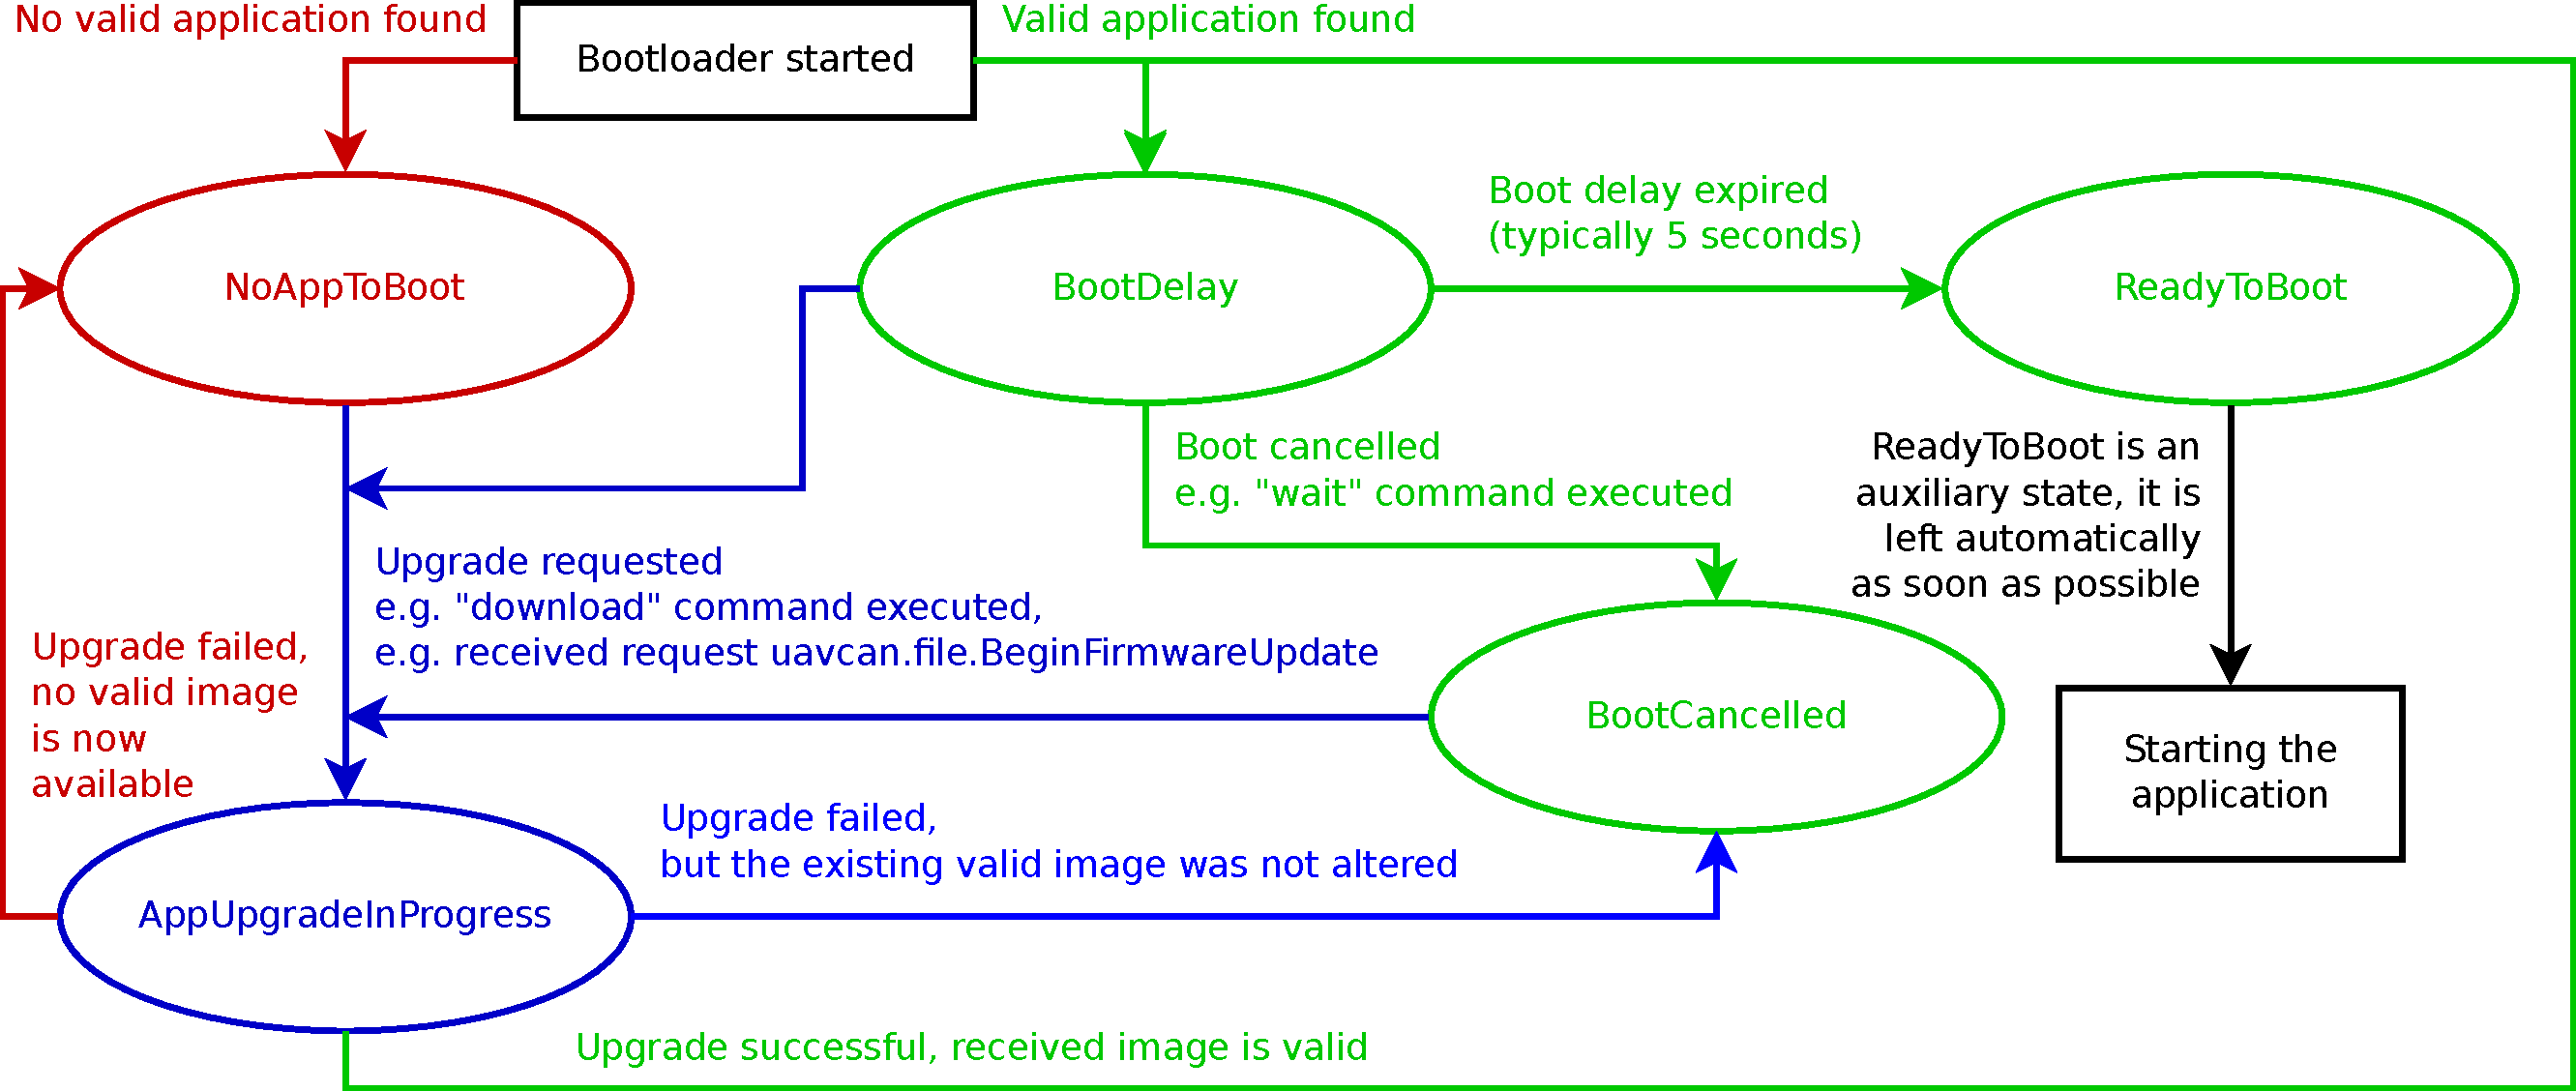
\includegraphics[width=\textwidth]{bootloader_state_machine}}
	\caption{Bootloader state machine.\label{bootloader_state_machine}}
\end{figure}

\begin{ZubaxSimpleTable}{Bootloader states}{|c l X|}\label{table:bootloader_states}
    ID & Name                 & Description \\

    0  & NoAppToBoot          & There is no valid application to boot;
                                the bootloader will be waiting for commands forever.\\

    1  & BootDelay            & The bootloader will start the application in a few seconds,
                                unless booting is canceled or a firmware update is requested.\\

    2  & BootCancelled        & There is a valid application to boot; however,
                                booting was canceled by an external command.\\

    3  & AppUpgradeinProgress & Application is currently being upgraded.
                                If interrupted, the bootloader will switch into
                                \textbf{NoAppToBoot} or \textbf{BootCancelled},
                                depending on whether there is a valid image after the interruption.\\
    
    4  & ReadyToBoot          & The application is about to boot.
                                This state is very transient and is left automatically as soon as possible.\\
\end{ZubaxSimpleTable}

\section{LED indication}

While the bootloader is running, the LED indicators behave as described in this section.

The status LED is always on, which is the main indicator that the bootloader,
rather than the application (firmware), is currently running.

The CAN1 LED behaves normally as a CAN bus activity and load indicator,
blinking once for 25 milliseconds every time the CAN1 controller successfully
transmits or receives a CAN frame.
Note that CAN frames that are filtered out by the hardware CAN acceptance filters
are not indicated by this LED.

The CAN2 LED displays one of the blinking patterns shown in the table \ref{table:bootloader_can2_led_behavior},
depending on which state the bootloader is in.
While the bootloader is running, the state of this LED has no relation to the state of
the redundant CAN interface (which is CAN2), since the bootloader makes no use of it.

\begin{ZubaxSimpleTable}{Bootloader state indicated via the CAN2 LED indicator}{|l l X|}
\label{table:bootloader_can2_led_behavior}
    Bootloader state         & LED pattern (step 50 ms) & LED behavior \\

    NoAppToBoot
    & \LEDX\LEDO\LEDX\LEDO\LEDX\LEDO\LEDX\LEDO\LEDX\LEDO\LEDX\LEDO\LEDX\LEDO\LEDX\LEDO\LEDX\LEDO\LEDX\LEDO
    & Blinking 10 Hz (very quickly) \\

    BootDelay, ReadyToBoot
    & \LEDO\LEDO\LEDO\LEDO\LEDO\LEDO\LEDO\LEDO\LEDO\LEDO\LEDO\LEDO\LEDO\LEDO\LEDO\LEDO\LEDO\LEDO\LEDO\LEDO
    & Turned off\\

    BootCancelled
    & \LEDX\LEDO\LEDO\LEDO\LEDO\LEDO\LEDO\LEDO\LEDO\LEDO\LEDO\LEDO\LEDO\LEDO\LEDO\LEDO\LEDO\LEDO\LEDO\LEDO
    & Blinking 1 Hz, short pulses (50 ms)\\

    AppUpgradeInProgress
    & \LEDX\LEDX\LEDX\LEDX\LEDX\LEDX\LEDX\LEDX\LEDX\LEDX\LEDO\LEDO\LEDO\LEDO\LEDO\LEDO\LEDO\LEDO\LEDO\LEDO
    & Blinking 1 Hz, long pulses (500 ms)\\
\end{ZubaxSimpleTable}

\section{Error codes}

The table \ref{table:bootloader_error_codes} provides descriptions for the well defined error codes
that can be reported by the bootloader.

\begin{ZubaxSimpleTable}{Bootloader error codes}{|r X|}\label{table:bootloader_error_codes}
    Code  & Description \\
        0 & Success.\\
        1 & Unknown error.\\
     9001 & Application ROM driver error: erase failed.\\
     9002 & Application ROM driver error: write failed.\\
    10001 & The current state of the bootloader does not permit the requested operation.\\
    10002 & Application image is too large for the device. Download has been aborted.\\
    10003 & Failed to write the next downloaded chunk of the application image into the ROM.\\
    20001 & X/YMODEM interface write has timed out.\\
    20002 & X/YMODEM retries exhausted.\\
    20003 & X/YMODEM protocol error.\\
    20004 & X/YMODEM transfer has been canceled by the remote.\\
    20005 & X/YMODEM remote has refused to provide the file.\\
    30001 & UAVCAN service request has timed out.\\
    30002 & UAVCAN file downloading has been interrupted.\\
    32767 & Unknown error.
\end{ZubaxSimpleTable}

\section{USB and UART interfaces}

This section is applicable to the serial interfaces exposed by the bootloader: USB and UART.

\subsection{Interface selection}

Once started, the bootloader launches a CLI\footnote{Command line interface.} instance on the UART port.
If the bootloader detects that the USB interface became active (by virtue of being connected to a USB host),
it disconnects the CLI from UART, rendering the latter silent and unresponsive,
and connects the same CLI to USB virtual serial port.
The CLI will remain available on the USB virtual serial port as long as the USB interface is active.
Shall the USB port become disconnected, the bootloader will switch the CLI back to UART.
The switching between USB and UART is fully automatic and happens on the fly.

Note that the bootloader may continue to report diagnostic messages via UART even
if the USB interface is currently used for communication.

\subsection{USB interface properties}

The USB interface will be detected by the host as CDC ACM (also known as virtual serial port).
This is a standard USB class that is supported by vast majority of operating systems out of the box,
no special drivers are required.

When the bootloader is connected via USB, it will be detected with the following properties:
\begin{itemize}
    \item Vendor ID -- 0x1D50
    \item Product ID -- 0x60C7
    \item Vendor string -- \verb|Zubax Robotics|
    \item Device description string -- \verb|Zubax GNSS Bootloader|
    \item Device ID -- the 128-bit globally unique device ID (section \ref{sec:product_identification})
                       as a hexadecimal string
\end{itemize}

\subsection{UART interface properties}

The UART interface has the following properties that cannot be changed:
\begin{itemize}
    \item Baud rate -- 115200
    \item Word size -- 8 bit
    \item Parity control -- none
    \item Stop bits -- 1
\end{itemize}

\subsection{CLI properties}

The CLI uses the CR-LF line ending sequence (\verb|\r\n|).
Remote echo and remote line editing are supported.

The CLI prompt has the following format:

\verb|StateName> |

The prompt always contains a human readable name of the current state of the bootloader
(see table \ref{table:bootloader_states}),
followed by the ASCII greater character ``\verb|>|'' (ASCII code 62), followed by a whitespace character.
For example:

\verb|BootDelay> |

Such prompt allows the user (or software) to easily identify the current state of the bootloader.

\subsection{CLI commands}

This section documents the CLI commands that can be of interest to the end user.
Some commands that are not intended for use in production are intentionally omitted from this reference.

\subsubsection{reboot}

Restarts the bootloader normally.

\subsubsection{wait}

Instructs the bootloader to not boot the application automatically.

If the current state is \verb|BootDelay|, the state will be switched to \verb|BootCancelled|.
In all other states the command will have no effect.

\subsubsection{download}

Instructs the bootloader to start an YMODEM/XMODEM/XMODEM-1K receiver on the current serial link
and await for the remote host to begin transmission of the new firmware binary image file.

The bootloader will automatically detect which file transfer protocol to use.

According to the YMODEM specification, if no transfer was initiated by the host within one minute,
the command will exit with an error.
Possible error codes are defined in the table \ref{table:bootloader_error_codes}.

Note that while this command is running, the CLI will be unavailable,
because the same serial link will be temporarily occupied by the file transfer protocol.
Automatic switching between USB and UART is not available while the command is running.

See the section \ref{sec:bootloader_ymodem_implementation} for the detailed information about the implementation.

\subsubsection{zubax\textunderscore{}id}

This is a standard command documented in the section \ref{sec:cli_command_zubax_id}.
Its implementation in the bootloader, however, has a number of additional features.

The firmware version information provided in the output is specific to the application image that is
installed on the device.
If the bootloader could not detect any application image on the device,
the firmware version fields will be omitted from the
output.\footnote{Version 1.0 of the bootloader used to employ a different convention where the application
version fields were using a different prefix: \texttt{fw\_} rather than \texttt{sw\_}.}

The version of the bootloader itself is reported via the following set of dedicated fields:
\begin{itemize}
    \item \verb|bl_version| -- bootloader version, major and minor, formatted as \verb|<major>.<minor>|
    \item \verb|bl_vcs_commit| -- bootloader version control system commit identifier as an integer number.
    \item \verb|bl_build_date| -- the build date of the bootloader.
\end{itemize}

An additional field named ``\verb|mode|'' is set to the string ``\verb|bootloader|''
to indicate that the bootloader is running rather than the application.

The table \ref{table:bootloader_zubax_id_fields} summarizes the fields reported by the bootloader.
Some extra fields may be reported as well,
which are not documented here because they are not designed for production use.

\begin{ZubaxSimpleTable}{Zubax ID fields}{|l X|}\label{table:bootloader_zubax_id_fields}
Field name              & Meaning \\

\texttt{product\_id}    & Product type identifier string.
                          The same string is reported via UAVCAN as the node name string. \\

\texttt{product\_name}  & Human-readable product name. \\

\texttt{mode}           & Set to the string ``\texttt{bootloader}'' to indicate that the bootloader is running. \\

\texttt{sw\_version}    & Application version number in the form ``major.minor''.
                          Omitted if the application could not be found. \\

\texttt{sw\_vcs\_commit}& Application version control system commit identifier.
                          Omitted if the application could not be found. \\

\texttt{hw\_version}    & Hardware version number in the form ``major.minor''. \\

\texttt{hw\_unique\_id} & The 128-bit unique ID of this specific hardware instance
                          (section \ref{sec:product_identification}).\\

\texttt{hw\_signature}  & The certificate of authenticity (CoA) of this specific hardware instance
                          encoded in a Base64 string.
                          \textbf{If this data is missing, please inform Zubax Robotics as soon as possible.} \\

\texttt{bl\_version}    & Bootloader version number in the form ``major.minor''. \\

\texttt{bl\_vcs\_commit}& Bootloader version control system commit identifier. \\
\end{ZubaxSimpleTable}

\subsection{YMODEM/XMODEM/XMODEM-1K implementation details}\label{sec:bootloader_ymodem_implementation}

YMODEM, XMODEM, and XMODEM-1K are simple and popular file transfer protocols designed by
Ward Christensen and Chuck Forsberg.
You can learn more about these protocols in the Zubax Knowledge Base at \url{https://kb.zubax.com/x/ZwAz}.
This section elaborates on the noteworthy implementation details specific to this application.

The \verb|download| command starts a multi-protocol receiver.
The receiver enters a loop where it emits the NAK character to the host,
prompting it to begin transmission of the firmware image file.
The receiver will emit NAK every 5 seconds until the host begins the transmission,
until the transfer initialization times out,
or until the host cancels the transmission, whichever happens first.
The transfer initialization timeout is set to 1 minute.

The receiver always uses the NAK character to initiate transfers rather than ``\verb|C|'',
which instructs the remote host to use the plain 8-bit checksum for data integrity protection
rather than CRC-16.
The data integrity guarantees offered by the plain 8-bit checksum algorithm are deemed sufficient,
because the data links are considered reliable enough,
and the firmware image itself is always protected by a strong CRC function.

Being compatible with three different protocols, the receiver supports the following options:
\begin{itemize}
    \item The host is free to send the zero block with file metadata, as defined by YMODEM.
          The receiver will collect the file size from the metadata packet and ignore the rest.
    
    \item The host is free to use either 256-byte or 1024-byte sized blocks, the receiver supports both.
          The former are defined by YMODEM and XMODEM, the latter are defined by YMODEM and XMODEM-1K.
\end{itemize}

Note that if the size of the firmware image file has not been provided,
the written image will be padded up to the size of the last data block.
This is acceptable, because the trailing bytes after the firmware image are
not used by any part of the system, and as such their contents can be arbitrary.
It is recommended, however, to fill the padding bytes with 0xFF,
in order to match the initial state of flash memory.

There is a large number of software products and scripts that support these file transfer protocols.
For instance, the popular program \verb|sz| (available on most GNU/Linux distributions) can be used as follows
(where \verb|$file| is the name of the firmware file, and \verb|$port| is the name of the serial port):
\begin{minted}[linenos = false]{bash}
sz -vv --ymodem --1k \$file > \$port < \$port
\end{minted}
There are various GUI-based alternatives for Windows and Mac OS as well.

\section{CAN bus interface}

\subsection{Overview}

The CAN bus interface is available on the CAN1 port only.
The CAN2 port is not used by the bootloader in any way.
It is one of the reasons why only the CAN1 port must be used
in deployments with non-redundant CAN buses.

The bootloader implements the UAVCAN firmware update protocol.
A detailed specification of the UAVCAN protocol in general and the firmware update part of it is available
on the official website at \url{http://uavcan.org}.

\subsection{Node status reporting}\label{sec:bootloader_uavcan_node_status}

The table \ref{table:bootloader_uavcan_status} describes the mapping from the bootloader states
to UAVCAN node status codes, as reported via the standard message \verb|uavcan.protocol.NodeStatus|.

The vendor specific status code field of the message contains the error code of
the last attempt to upgrade the firmware.
The error codes are documented in the table \ref{table:bootloader_error_codes}.

The message is broadcasted at a fixed interval of 1 second.
Out-of-order messages may be emitted when the status of the bootloader changes.

\begin{ZubaxSimpleTable}{Bootloader states and UAVCAN node status codes}{|l X X|}
\label{table:bootloader_uavcan_status}
    Bootloader state       & UAVCAN node mode   & UAVCAN node health\\
    NoAppToBoot            & SOFTWARE{\_}UPDATE & ERROR \\
    BootDelay, ReadyToBoot & MAINTENANCE        & OK \\
    BootCancelled          & MAINTENANCE        & WARNING \\
    AppUpgradeInProgress   & SOFTWARE{\_}UPDATE & OK \\
\end{ZubaxSimpleTable}

\subsection{Node identification}\label{sec:bootloader_uavcan_node_identification}

The service \verb|uavcan.protocol.GetNodeInfo| is responded to as follows.

If the bootloader was able to detect a valid application (i.e. firmware) image on the device,
all fields of the nested structure \verb|uavcan.protocol.SoftwareVersion|
(which are \verb|major|, \verb|minor|, \verb|vcs_commit|, and \verb|image_crc|)
will be populated with the information obtained from the application image.
If no valid application image could be found, the fields will be zeroed.

The fields \verb|uavcan.protocol.HardwareVersion| and \verb|name|
are always populated as described in the section \ref{sec:uavcan_node_identification}.

\subsection{Node restarting}\label{sec:bootloader_uavcan_node_restarting}

The service \verb|uavcan.protocol.RestartNode|, if the provided magic number is correct,
unconditionally reboots the device.
If the provided magic number is incorrect, the device returns a response with the field \verb|ok|
set to zero (false).

\subsection{Node initialization}

The bootloader is a full plug-and-play UAVCAN node that requires no initial configuration prior to
use.\footnote{If that were not the case, the device would have been easy to brick
by uploading an invalid firmware and then turning the power off.}

\subsubsection{CAN bus bit rate detection}

Once started, the bootloader will automatically detect the bit rate of the CAN bus it is connected to
(if connected to any at all), and remember the detected bit rate for the rest of its work.
There is no detection timeout, which means that the bootloader can be connected to a CAN bus at
any moment while running, and it will configure itself immediately.

If the bit rate has been detected successfully, its value will be passed over to the application
during the booting, so that the application won't have to perform the bit rate detection again.

Note that if the bootloader was started from the application,
and at the time of it the application knew the bit rate of the CAN bus,
the value will be supplied to the bootloader.
In this case the bootloader will use the provided bit rate value and skip the detection procedure.

The bootloader requires up to approximately 4 seconds to perform the bit rate detection on a properly
functioning CAN bus.
If the bus is exhibiting erroneous behavior, the bootloader may need a longer time to complete the bit rate
detection procedure.
The list of supported bit rates is provided below:
\begin{itemize}
    \item 1 Mbit/s
    \item 500 kbit/s
    \item 250 kbit/s
    \item 125 kbit/s
\end{itemize}

\subsubsection{Node ID allocation}\label{sec:bootloader_uavcan_node_id_allocation}

After the CAN bus bit rate is established, the bootloader will request a dynamic UAVCAN node ID from the bus.

If the node ID has been obtained successfully, its value will be passed over to the application
during the booting, so that the application will be able to re-use it.

Note that if the bootloader was started from the application,
and at the time of it the application's own UAVCAN node had a valid node ID,
the value will be supplied to the bootloader.
In this case the bootloader will use the provided node ID and skip the allocation procedure.

Until there is a valid node ID available for the bootloader,
no other functions of the UAVCAN interface will work.

\subsection{Firmware update process}

\subsubsection{Waiting for the update request}\label{sec:bootloader_uavcan_begin_update_request}

In order to be able to begin downloading the new application image over UAVCAN,
the bootloader needs to know the following two parameters:
\begin{itemize}
    \item The UAVCAN node ID of the remote node that contains the application image file
          that should be downloaded.

    \item The file system path to the application image file within the remote node.
\end{itemize}

The above listed parameters can be supplied to the bootloader in two ways:
\begin{itemize}
    \item By calling the standard UAVCAN service \verb|uavcan.protocol.file.BeginFirmwareUpdate|
          while the bootloader is running.
          The request payload of that service contains the necessary data.
          
    \item By the application. This is the case when the application receives the above request
          and passes the parameters from it directly to the bootloader when rebooting into it.
          In this case the bootloader skips this step and proceeds straight to the next one.
\end{itemize}

\subsubsection{Downloading the application image}\label{sec:bootloader_uavcan_file_transfer}

At this stage, the bootloader has all of the information required to begin the actual update process.

The standard service \verb|uavcan.protocol.file.Read| is emitted in a loop in order to transfer
the contents of the new application image to the device.
The transfer priority is set to 24 (low).
The service response timeout is set to 1 second (the default recommended by the UAVCAN specification).

In order to avoid congestion of the CAN bus while the file transfer is in progress,
the bootloader inserts a delay after completion of each file read service invocation.
The delay is a function of the CAN bus bit rate, and it is defined as follows
(the bit rate unit is bit/second):

$$\frac{1}{1 + {\text{can{\_}bus{\_}bit{\_}rate}}/{65536}}$$

Some of the practical values are listed below for reference:
\begin{description}
    \item[1 Mbit/s] -- 62 ms
    \item[500 kbit/s] -- 116 ms
    \item[250 kbit/s] -- 208 ms
    \item[125 kbit/s] -- 344 ms
\end{description}

While the file transfer is in progress,
the bootloader will be reporting its progress several times per minute
by emitting human-readable log messages,
as described in the section \ref{sec:uavcan_bootloader_logging}.

A log message will also be emitted at the end of the process in order to indicate whether it was successful,
and if not, what was the reason of the failure.

\subsection{Logging}\label{sec:uavcan_bootloader_logging}

The bootloader aperiodically broadcasts human-readable log messages using the standard UAVCAN type
\verb|uavcan.protocol.debug.LogMessage| at the lowest transfer priority level.
Some of the important logging points include the following:
\begin{itemize}
    \item File transfer progress report.
    \item Update completion -- whether successful or not, reason for the failure, if applicable.
\end{itemize}

\subsection{Data type summary}

\begin{ZubaxSimpleTable}{Broadcasted UAVCAN messages}{|l l l X|}
    Data type name                                        & Period     & Transfer priority & Section \\

    \texttt{uavcan.protocol.NodeStatus}                   & 1 \& ad-hoc
                                                          & 24 (low)
                                                          & \ref{sec:bootloader_uavcan_node_status}\\

    \texttt{uavcan.protocol.dynamic\_node\_id.Allocation} & Aperiodic
                                                          & 30 (low)
                                                          & \ref{sec:bootloader_uavcan_node_id_allocation}\\

    \texttt{uavcan.protocol.debug.LogMessage}             & Aperiodic
                                                          & 31 (lowest)
                                                          & \ref{sec:uavcan_bootloader_logging}\\
\end{ZubaxSimpleTable}

\begin{ZubaxSimpleTable}{Subscribed UAVCAN messages}{|l X|}
    Data type name                                        & Section \\
    \texttt{uavcan.protocol.dynamic\_node\_id.Allocation} & \ref{sec:bootloader_uavcan_node_id_allocation}\\
\end{ZubaxSimpleTable}

\begin{ZubaxSimpleTable}{UAVCAN service servers}{|l X|}
    Data type name                                        & Section \\
    \texttt{uavcan.protocol.GetNodeInfo}                  & \ref{sec:bootloader_uavcan_node_identification}\\
    \texttt{uavcan.protocol.RestartNode}                  & \ref{sec:bootloader_uavcan_node_restarting}\\
    \texttt{uavcan.protocol.file.BeginFirmwareUpdate}     & \ref{sec:bootloader_uavcan_begin_update_request} \\
\end{ZubaxSimpleTable}

\begin{ZubaxSimpleTable}{UAVCAN service clients}{|l l l X|}
    Data type name                     & Response timeout & Transfer priority & Section \\
    \texttt{uavcan.protocol.file.Read} & 1 second
                                       & 24 (low)
                                       & \ref{sec:bootloader_uavcan_file_transfer} \\
\end{ZubaxSimpleTable}

\end{document}
